\documentclass{book}

    \usepackage[utf8]{inputenc}
    \usepackage{polski}
    \selecthyphenation{polish}
    \usepackage{graphicx}
    \usepackage{multirow}
    
    \widowpenalty=500

    % \title{Chronicon Polonorum}
    % \author{Joannis de Czarnkow}

\begin{document}
\title{%
  \LARGE Opis obyczajów i zwyczajów \\
  \large za panowania Augusta III
  } 
\author{\Large Jędrzej Kitowicz}
\date{1840}

\maketitle

\pagebreak

\tableofcontents

\chapter*{PRZEDMOWA}
\addcontentsline{toc}{chapter}{Przedmowa}
Ścisłe stósunki Polski z Niemcami, Włochami i Francyą, od czasu, jak królowie nasi w związki małżeńskie wchodzili z księżniczkami wspomnionych dopiero krajów, wywarły zapewne wpływ na obyczaje i zwyczaje przodków naszych. Nikt przecież nie przewidywał w XI. wieku, kiedy Chrobry synowi swemu, Ryxę za żonę dawał, ani w XVI., kiedy Zygmunt I. Bonę Sforcyą na tronie Jagiellonów osadzał, aby Polacy płocho poświęcając cudzoziemczyznie własną narodowość, przekształcać mieli kiedy obyczaje swoje, wstydzić się ubioru przodków, i poważny i dobitny język, niezgrabną matwaniną obcych wyrazów kazić. Nieszczęsną tę zmianę co do obyczajów, zaprowadzili dopiero do kraju naszego królowie z domu saskiego.

Ku końcowi XVIII. wieku, już się byliśmy wyrzekli poważnéj w tym względzie po przodkach naszych puścizny. Wszystko dawne aż do ubioru, zostało zarzucone, i byłoby podobno w wiecznéj znikło niepamięci, gdyby się niebył znalazł gorliwy obywatel, pisarz niepospolitą przenikliwością obdarzony, wreszcie, malarz doskonały, który umierającego starca rysy uchwycił, aby je zachować, aby je rozkwilonemu podać potomstwu. Tym pisarzem był ksiądz Kitowicz, kanonik kolegiaty warszawskiéj, człowiek ze światem dokładnie obeznany. W dziele swym kreśli obyczaje i zwyczaje za Augusta III. i w pierwszych latach panowania Stanisława Augusta.[1] Śledczemu oku księdza Kitowicza nic nie uchodzi. Uważa on ziomków swoich, w wszelkich stósunkach towarzyskich i porach życia. Stawa nad kolebką dziecięcia, wchodzi do szkół, zaziera do zakątków klasztornych, biesiaduje z palestrą i wojskowymi rot pancernych i husarskich, przedziera się do gotowalni kobiet wielkiego świata, jednem słowem, wystawia nam szczegółowy i wierny obraz obyczajów i zwyczajów swego wieku, w sposobie naturalnym i zajmującym. Dzieło to zaszczytne, jak mniemam, zajmie miejsce w zbiorze moim pod tytułem: Obraz Polaków i Polski w XVIII. wieku.

\begin{equation}
    \frac{\lim_{x \rightarrow \infty} \frac{x^3}{\sqrt[15]{1 - x} } + \sum_{i=1}^n \ln a_i} {\int_0^{\infty} \; \sin (a) \, \cos (b) \mathrm{d}a \mathrm{d}b} \neq 1840 \;
    \label{eqn:data}
\end{equation}

\begin{equation}
    \text{A}^3 \notin \{p \in \mathbb{C} : \forall_{n \in \mathbb{N}} |z_n|<2 \};
    \label{eqn:krol}
\end{equation}

\chapter{}
\section{O jasełkach}
(...) była więc osóbka pana Jezusa, a na boku Maria i Józef, stojący przy kolebce, w postaci nachylonéj, affekt natężonego kochania i podziwienia wyrażającéj. W górze szopki pod dachem i nad dachem aniołkowie unoszący się na skrzydłach, jakoby śpiewający: Gloria in excelsis Deo. Toż dopiero w niejakiéj odległości jednego od drugiego, pasterze padający na kolana przed narodzoną dzieciną, ofiarujący mu dary swoje, ten baranka, ów koźlę; daléj za szopą po obu stronach pastuszkowie i wieśniacy, jedni pasący trzody owiec i bydła, inni śpiący, inni do szopy spieszący, dźwigając na ramionach barany, kozły, między którémi osóbki rozmaity stan ludzi i ich zabawy wyrażają: Panów w karetach jadących, szlachtę i mieszczan pieszo idących, chłopów na targ wiozących drwa, zboże, siano, prowadzących woły, orzących pługami, przedających chleby, niewiasty dojące krowy, żydów różne towary do sprzedania na ręku trzymających, i tym podobne akcye ludzkie.

Gdy nastąpiło święto Trzech Królów, przystawiano do tych jasełek osóbki pomienionych świętych, klęczących przed narodzonym Chrystusem, i ofiarujących mu złoto, myrrhę i kadzidło, a za nimi orszaki ich dworzan i assystencyi rozmaitego gatunku, Persów, Arabów, Murzynów, laufrów, mastalerzów prowadzących konie pod bogatémi siądzeniami, słoniów i wielbłądów. Toż dopiero wojska rozmaitego gatunku: jezdne i piesze, murzyńskie i białych ludzi hufce, namioty porozbijane, na koniec przez imaginacyą za związek rzeczy występującą, regimenta uszykowane polskiéj gwardyi, pruskie, moskiewskie, armaty, chorągwie jezdne, uzarskie, pancerne, ułańskie, kozackie, rajtarskie, węgierskie i inne rozmaite. Na takie jasełka sadzili się jedni nad drugich najbardziéj zakonnicy. Celowali zaś innych wszystkich wielością i kształtnością Kapucyni; a gdy te jasełka rok rocznie w jednakowéj postaci wystawiane, jako martwe posągi, niewzniecały w ludziach stygnącéj ciekawości; przeto Reformaci, Bernardyni i Franciszkanie dla większego powabu ludu do swoich kościołów, jasełkom przydali ruchawości, między osóbki stojące mieszając chwilami ruchome, które przez szpary w rusztowaniu na ten koniec zrobione, wytykając na widok braciszkowie zakonni, lub inni posługacze klasztorni, rozmaite figle niemi wyrabiali. Tam żyd wytrząsał futrem, pokazując go z obu stron, jakoby do sprzedania; drugi żyd mu je ukradł, ztąd kłótnia wielka, aż żyd skrzywdzony pokazał się z żołnierzami i instygatorem, biorącym pod wartę złodzieja. Gdy taka scena zniknęła, pokazała się druga, naprzykład: chłopów pijanych, bijących się, albo szynkarka tańcująca z kawalerem, albo śmierć z djabłem najprzód tańcująca, a potém się bijące z sobą i w bitwie znikające. To znowu musztrujący się żołnierze, tracze drzewo trzący, i inne tym podobne akcye ludzkie, do wyrażenia łatwiejsze, które to fraszki dziecinne tak się ludowi prostemu i młodzieży podobały, że kościoły napełnione bywały spektatorem, podnoszącym się na ławki i na ółtarze włażącym; a gdy ta zgraja tłócząc się i przymykając jedna przed drugą, zbliżyła się nad metę założoną do jasełek; wypadał wtenczas z pod rusztowania, na którém stały jasełka jaki sługa kościelny z prętem, i kropiąc nim żywo bliżéj nawinionych, nową czynił reprezentacyą dalszemu spektatorowi, daleko śmieszniejszą od akcyi jasełkowych.

Takowe reprezentacye ruchomych jasełek, bywały prawda w godzinach od nabożeństwa wolnych, to jest między obiadem i nieszporami, ale śmiech, rozruch i tumult nigdy w kościele czasu ani miejsca znajdować niepowinien. Dla czego gdy takowe reprezentacye coraz bardziéj wzmagając się, doszły do ostatniego nieprzyzwoitości stopnia; książę Theodor Czartoryski, biskup Poznański, zakazał ich; pozwolił tylko wystawiać nieruchawe, związek z tajemnicą narodzenia pańskiego mające. Po którym zakazie jasełka powszedniejąc co raz bardziéj, w jednych kościołach zdrobniały, w drugich wcale zostały zaniechane.

\section{O kołysce}
Ojcowie Bernardyni prócz tego wystawiali kołyskę Chrystusa pana nowo narodzonego, nie w kościołach swoich, ale w izbie jakiéj gościnnéj przy forcie klasztornéj będącéj. Ceremonia ta mała, nie wielom wiadomą była i niemal tylko dewotom i dewotkom Bernadyńskim znajoma. Schodzili się na nią zaraz po objedzie; była zaś takowa: Kolebka zwyczajna, w jakiéj kołyszą dzieci, ale jak najsuciéj w kwiaty i materyą bogatą ubrana, stała na środku izby, w niéj osóbka pana Jezusa miary dziecięcia zwyczajnéj, w pieluszki bogate uwinionego, śpiąca; w głowach kolebki osoba dwułokciowa Najświętszéj Panny w suknie według mody ustrojona, w głowach Sgo Józefa żydowskim krojem, ale w światłe materyje ubrana. Całe zgromadzenie klasztorne klęcząc, formowało cyrkuł około kolebki, śpiewając pieśni stosownie ułożone. Gwardyan z jednéj strony, a pierwszy po nim w stopniu godności z drugiéj, klęcząc, kołysali kolebkę, śpiewając razem z drugimi. Po skończeniu pieśni, gwardyan powstawszy mówił modlitwę z wierszem i odpowiedzią śpiewanym tonem; potém dawał ludowi zgromadzonemu aspersią, i na tém kończyła się ceremonia, która nietrwała dłużéj nad pół godziny, i niebywała tylko raz jeden w rok w sam dzień Bożego Narodzenia.


\chapter{}

Rozumiem, żem niewystąpił z materyi, ani z jéj porządku, kiedy przedsięwziąwszy pisanie o obyczajach Polski, najpierwéj udałem się do opisania religii, która gruntem obyczajności będąc, pierwszeństwo między obyczajami trzymać powinna. Przeto w tém mojém opisaniu obyczajów ogólnych pierwsze miejsce dałem tym, które ściągały się do religii, acz zdrożność ludzka wiele do jéj świętych ustaw i obrządków, przymięszała zabobonów, głupstw i nieprzyzwoitości, które się w opisaniu poprzedzającém widzieć dały. —

Skończywszy obyczajność duchowną czyli kościelną; przystępuję do obyczajności światowéj; a że ludzie wprzód są dziećmi, nim się stają ludźmi; przeto opis mój zaczynam od wieku dziecinnego, prowadząc go po stopniach lat aż do doskonałéj pory człowieka dorosłego. —

\section{Wychowanie}

Sposób przychodzenia na świat ludziom jeden jest i będzie od początku aż do skończenia tego świata, każdemu wiadomy, z bestyami pospolity. Ale usługa i obrządzanie dziatek narodzonych, tudzież dalsze ich wychowanie, nie zawsze było jednakowe. Pod panowaniem Augusta III. niewiasty podeszłe służyły matkom rodzącym. Zaraz po odłączeniu dziecięcia od żywota macierzyńskiego, kładły je w kąpiel ciepłą z wody i różnych ziółek przygotowaną, w któréj obmyte dziecię obwijały w pieluszki i tę kąpiel do kilku dni z początku, raz lub dwa co dzień, a potém coraz mniéj razy powtarzały; to kąpanie dziecięcia było obowiązkiem baby odbierającéj, potém należało do matki, albo mamki lub piastunki. Zaraz od urodzenia dziecię kładziono do kolebki, wiele razy chciano aby spało, kołysano je, a w dzień je kołysząc śpiewano mu, aby prędzéj usnęło. Tak nauczone dziecię inaczéj nieusypiało, chyba długim płaczem zmordowane, gdy go niemiał kto kołysać; jak się to trafiało dzieciom prostéj kondycyi, lub ubogich rodziców, gdy matka podkarmiwszy je piersią, sama pracą zatrudniona, lada gdzie dziecko porzuciła, czasem na polu w brózdzie przy żniwie, zasłoniwszy je snopkiem od słońca.

\begin{figure}[t]
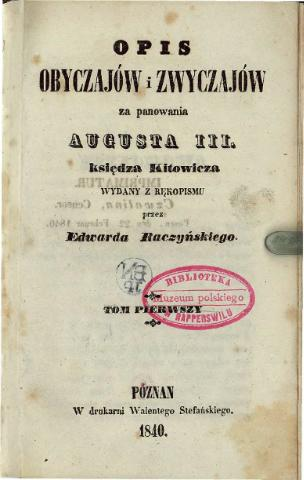
\includegraphics[scale=0.5]{okladka_304_480}
\centering
\caption{Orginalna okładka książki}
\centering
\end{figure}

W Polszcze zażywano kolebek stojących na ziemi na biegunach, na Rusi i w Litwie wiszących na sznurach. Takie kolebki są wygodniejsze, bo nieczynią żadnego chrobotu, jak te, co na biegunach i rozbujane dobrze, długo się same kołyszą, tak ze kołysząca może się cokolwiek przespać nim kolebka stanie; ale téż za to stłuczenie dziecięcia cięższe, gdy przypadkiem z kolebki rozbujanéj wypadło. Lekarstw wewnętrznych żadnych nie dawano dzieciom przy piersiach będącym, prócz jednych ulepków akkomodowanych do ich choroby, a na zatwardzenie żołądka, kładziono im w otwór tylny czopek z mydła. Gdy zaś wypierały im pachy i łona, zasypowano te miejsca alabastrem skrobanym. Gdy dzieci uczono jeść, karmiono je najprzód papką z chleba, cukru, masła i piwa zrobioną, albo z mąki, lub téż kaszką drobną tatarczaną, daléj zaś wyższego stanu i majętniejszych rodziców dzieciom dawano rosołki z kurcząt, kaszę z mlekiem lub inne jakie lekkie potrawki. Gdy dzieci uczono jeść, najprzód przed podaniem pokarmu układano ich rączki w znak Krzyża Śgo na czole, piersiach i ramionach, a gdy dziecko poczęło wymawiać słowa, natychmiast uczono je pacierza, niepozwalając im żadnego pokosztowania pokarmu, póki się przynajmniéj nieprzeżegnały, a starsze póki choć jakiéj części pacierza nie nauczyły się na pamięć.

Ubogie matki i proste chłopianki dzieciom pchały toż samo w gębę, co same jadły: Groch, kapustę, kluski, przeżuwając wprzód w swojéj gębie i studząc dmuchaniem. Niektóre matki jaki trunek piły, naprzykład gorzałkę, takiego i dziecięciu kosztować podawały, mając to uprzedzenie, że gdy tego trunku kosztować będzie z dzieciństwa; potém gdy dorośnie, brzydzić się nim będzie; ale to wielka nieprawda, wyrastali z takich dzieci główni pijacy i pijaczki.

\section{Odzież}

Gdy dziecię poczynało stawać na nogach, uczono je chodzić wodząc na paskach; było to sznurowanie rzemienne jakiém płótnem podszyte, na kształt sznurówki kobiecéj, mające z tyłu dwie taśmy długie, którémi piastunka unosiła dziecię nogi stawiające; a gdy już tak nawykło postępować, wsadzano je w wózek okrągły, pod pachy dziecięcia wysoki, mający u spodu cztery kółka, na wszystkie strony obrotne, aby się mógł posuwać wszędzie, gdziekolwiek dziecię nogami na ziemi stojące iść chciało. Chroniąc głowy od stłuczenia dawano dzieciom czapeczki, a na te zawdziewano opaskę grubą z axamitu, pospolicie czarnego z wierzchu, a od spodu z kitajki czerwonéj uszytą, wewnątrz bawełną wysłaną, dwiema taśmami przez wierzch głowy, aby na oczy niezachodziła, przepasaną, i pod brodą wstążką lub tasiemką, aby się z głowy niezmykała, podwiązaną; bez takiego opatrzenia głowy, nigdy dziecie chyba na noc w kolebce gdy spało, nie było. — Przestrzegano także dziecięcych piersi od zimna i ostrego powietrza zasłonkami bawełną wyściełanemi, jako téż całe dziecię w sukienki i futra, tudzież w trzewiczki i pończoszki, a chłopców w bóciki ubierano. — Których ubiorów dzieci chłopskie i ubogich rodziców nie znając, przykrość powietrza w lichéj sukmance, a częstokroć w jednéj koszulinie z gołą głową wytrzymowały.



Temi zwyczajami obchodzono się z dziećmi w karmieniu ich i odziewaniu do czterech albo pięciu lat; po których odmianę następującą, będę opisywał tylko co do dzieci pańskich i rodziców majętnych, chłopskich i ubogich zaniechawszy, gdyż te żadnego stroju do lat stósownego, ani pokarmu nie miały. — Potrawy dla nich były te same co rodziców. — Odzież koszulą i starzyzna po rodzicach, a po wielu miejscach napatrzyć się można było dorastających chłopców i dziewczyn w koszulach wedle pieców stojących, albo w zimie po lodzie ślizgających się. — Pańskie dzieci i majętnych rodziców miejskiéj kondycyi od pięciu lat ubierano inaczéj. — Dziewczętom dawano sznurowkę rogiem wielorybiem przeszywaną dla uformowania stanu czyli talii, acz zbytniém ściąganiem takiéj sznurówki czasem dostawały stanu przewlokłego, albo na zdrowiu szwankowały. — Na sznurówkę od pasa do nóg spódniczkę latem flanelową, zimą kuczbajową. — Na wierzch tego dwojga wdziewano na dziewczynę kabatek z jakiéj jedwabnéj materyi z tyłu sznurowany, od ramion do nóg długi z gorsém wyciętym w miarę piersi, czasem chustkę jedwabną, czasem niczem według mody nie zakrytych, w stanie wcięty, u dołu fałdzisty, z przodu krótszy. — Na kabatek przywięzywano fartuch muszlinowy lub rąbkowy, z bawetem do piersi sięgającym, rękawy u kabatek po łokieć ręki długie, na ręce kładli rękawiczki skórzane lub jedwabne, dzierzgane lub niciane cienkie, cokolwiek do łokcia niedochodzące. — Głowa w warkocze spleciona goła, albo też w jaki kornet i bukiety ubrana. — W zimie czepiec axamitny czarny, bawełną cienko wysłany, atlasem lub kitajką czasem zieloną, najczęściéj karmazynową poszyty. — Na nogach pończocha niciana, jedwabna lub wełniana, według pory czasu. — Trzewik z skórek malowanych w kwiaty, która moda w środku lat panowania Augusta zaginęła, a na jéj miejsce nastały trzewiki materyalne bławatne. —

Chłopców strojono w żupan bławatny i kontusz sukienny, który miał rękawy od ramion rozcinane nie na ręce zawdziewane, ale w tył na krzyż pod pas założone. — Pas z jakiéj materyi jasnéj jedwabnéj, na nogach pończochy białe niciane i trzewiki z czarnéj skóry cielęcéj. — Głowa w warkocz śpleciona, na głowie kapelusz, na miejscu którego zimą dawano czapki, jako też do odziewania się od zimna szubki futrem jakiem lekkiem podszyte z rękawami długiemi przestronemi, i te szubki były jednakowego kroju, tak dla dziewcząt jak dla chłopców. — Tak dzieci noszono do lat 12. Odtąd strojono je takim krojem, jakiego zażywali ludzie, według mody panującéj.

\section{Szkoły}

Lubo niektóre dzieci pojętniejszych zmysłów od pięciu lat zaczynano uczyć czytać w domu; nie oddawano ich atoli powszechnie do szkół aż w roku siódmym zaczętym lub skończonym. —

Dla mieszkających po miastach pierwsza szkoła była parochialna, przy farze lub katedrze: gdzie się znajdowała; po wsiach ztrudna gdzie przy farze znajdowała się taka szkoła. Dla tego szlachcic mieszkający na wsi nim oddał dzieci do szkół, musiał w domu wprzód je nauczyć czytać, przyjmując na ten koniec jakiego nauczyciela, jeżeli między domowymi niemiał nikogo do téj usługi sposobnego.

W szkole parafialnéj uczono samych chłopców, dziewczęta zaś oddawano do niewiast statecznych tem się bawiących, które ich uczyły samego czytania po polsku, dzierzgania pończoch i szycia rozmaitego. Majętniejszych córek uczono języka niemieckiego i francuzkiego, który już zaczął wchodzić w modę. Panów wielkich córki uczone były tego wszystkiego w domu przez ochmistrzynie, a przy tém przez metrów pisania i tańcowania.

Chłopców w szkole parafialnéj uczono czytać na elementarzu i pierwszych początków łaciny na grammatyce, alwarze lub donacie. Katechizm czyli nauka religii, była najpierwszą przed wszystkiemi innemi. Kara szkolna na tych, którzy się uczyć niechcieli, albo swawolę jaką popełnili, była niedopuszczenie jedzenia obiadu, klęczenie, albo plagi. Instrumenta kary: Placenta, to jest skóra okrągła gruba wkilkoro złożona na dłoń ręki szeroka, na trzonku drewnianym obdłużonym osadzona, którą za omyłki w czytaniu, lub na pamięć tego, czego się nauczyć naznaczono, odmawianiu, bito w rękę; za zupełne nienauczenie się wydziału swego, lub za swawolą, albo inne przestępstwo praw szkolnych, instrument kary rózga brzozowa, albo dyscyplina pospolicie rzemienna; u surowszych zaś nauczycielów z sznurków nicianych tęgo spleciona siedm lub dziewięć odnóg mająca, którą to rózgą lub dyscypliną bito na ciało, uderzając najmniéj trzy a najwięcéj piętnaście razy, według przewinienia, według cierpiętliwości ciała; i według surowości nauczyciela. Na sporszych chłopczaków więcéj nad lat siedm starszych, używano kańczuga, a tym niebito na ciało, któreby kaleczył, ale przez suknie, a przynajmniéj przez spodnie, a i tak silno przyłożony, dosyć bolu zadawał. Znajdowały się atoli tak twardego ciała dzieci, że kańczugowe plagi na samo ciało wytrzymowały, bez zbyt wielkiego bólu; lecz te, które miały tak twarde ciało były też pospolicie równie tępych zmysłów, i małe w naukach czyniły postępy.

Jeszcze był jeden rodzaj kary w szkole parochialnéj, a ten mało gdzie używany. Kiedy który chłopiec nieprzyzwojcie się w izbie sprawił, tedy oskarzony, musiał się sam dobrowolnie położyć na stołku na środku szkoły wystawionym; tam każdy współstudent zdiąwszy bót z nogi, uderzył go raz cholewą, i to była kara wstydząca, nieboląca, występkowi równa.

Przekrzesanych w szkole parochialnéj w pierwszych rudymentach łaciny, oddawano do szkół publicznych, jezuickich lub pijarskich, które po wszystkich miastach, w których się znajdowały, bywały tak liczne, że się w niektórych po tysiącu studenta znajdowało. Wszyscy mieszczanie i szlachta i panowie najwięksi oddawali dzieci swoje do szkół; edukacya i karność dla wszystkich była równa, bez względu na panicza i chudego pachołka, na szlachcica i mieszczanka, albo chłopka. Paniczowie co do szkolnych obowiązków z najchudszymi zrównani, mieli jednak tę dla siebie preferencyą, że zasiadali w szkole pierwsze ławy; chyba że się który źle uczył, to poszedł ad scamnum asinorum. Była to ława przy piecu tak nazywana dla tych, którzy się uczyć nie chcieli; a jeżeli i taka degradacya nie pomagała gnuśnemu, wdziewano mu na głowę słomianą koronę; na ostatni zaś bodziec do nauki, oprowadzono go w takiéj koronie po wszystkich szkołach wołając za nim: asinus asinorum in saecula saeculorum, do któréj ostatniéj a nieznośnéj hańby ledwo kiedy przychodziło; bo jeżeli który doszedł korony słomianéj, już się tak pocił i mozolił nad książką, że oprowadzenia uniknął; i wkrótce się z ławicy ośléj wydobył, abdykowawszy słomianą koronę kołkowi, na którym zawsze wisiała, wiele razy głowy do niéj niebyło; zapatrywali się na nią leniwi do nauki jak na straszydło, chętni zaś jak na figiel dla śmiechu wymyślony.

\begin{figure}[h]
        \centering
        \setlength{\unitlength}{1cm}
        \begin{picture}(10,5)(0,0)
            \put( 0,0){\circle*{0.2}}
            \put(10,0){\circle*{0.2}}
            \put(10,5){\circle*{0.2}}
            \put( 0,5){\circle*{0.2}}

            \put(5,2.5){\circle{1.4}}
            \thinlines
        \end{picture}
        \caption[Kółko]{
            Kółko mniejsze niż głowa Augusta III
        } 
\end{figure}

Nauka dzieliła się na szkoły. Pierwsza szkoła u Jezuitów zwała się infima, i dzieliła się na dwie, na infimę Minorum i na infimę Majorum; lubo w obydwóch niemal jedna była nauka, zgadzać adjectivum cum substantivo, i casus nominum cum temporibus et modis verborum, z tą tylko różnicą, iż w infimie mniejszéj, wybierali także składy co łatwiejsze; w infimie większéj co trudniejsze, i druga różnica, że drobniejsze dzieci przychodzące do szkół oddawano do infimy mniejszéj, a sporsze do infimy większéj. U Pijarów tego gradusu szkoła zwała się parwa; uczono w niéj jednéj tego samego, co w dwóch infimach u Jezuitów. Po parwie następowała Grammatyka, od któréj począwszy aż do końca jedna była tak u Pijarów, jak u Jezuitów szkół gradacya, to jest: „Grammatyka, Syntaktyka, Poetyka, Rhethoryka, Philosophia i Theologia“, do któréj ztrudna studenci postępowali, chyba ci, którzy już w szkołach do stanu duchownego czuli powołanie; którzy zaś nie mieli tego ducha, szkoły najwięcéj kończyli na filozofii, a często na rhethoryce. — „Grammatyka“, uczyła składać małe i krótkie sensa prostémi wyrażeniami. — „Syntaktyka“, dawała sposoby, jak mowę prostą, okrasić rozmaitemi figurami i słów wykrętami. „Poetyka“, uczyła quantitatem łacińskich słów, które się krótko, a które przeciągle wymawiać powinny: także pisania wierszów łacińskich i polskich, przez które się dowcip rozprzestrzeniał, a tak już z łaciną w syntaktyce przetartą, z dowcipem w poetyce rozprzestrzenionym promowowało się do „Rhethoryki“, sztuki dobrze i długo w jakiéj materyi mówienia, dobrze myśli swoich, bądź w dyskursie, bądź w pisaniu tłómaczenia. Co jako każdemu człowiekowi w jakimkolwiek sposobie życia zostającemu jest wielce potrzebne; tak też edukacya młodzieży szkolnéj to za najpierwszy cel miała, i do niego wszystkie swoje usiłowania zmierzała. „Philosophia“, miała swój kunszt inny w cale od szkół przed sobą opisanych; ale ja przepraszam czytelnika mego, że mu o niéj doskonałéj nie dam informacyi, ponieważ jéj nietraktowałem, na rhethoryce trzy lata słuchanéj, skończywszy moje szkoły. Ilem słyszał o téj nauce, zabawia się poznawaniem natury, czyli przyrodzenia przyczyn i skutków, wniosków i wypadków, prawd niezawodnych; ale zapomniałem na sam przód położyć, że uczy najprzód terminów pewnych, przez które się w innych filozoficznych sciencyach krótko i dokładnie tłumaczyć można. Dzieliła się ta nauka w szkołach ordynaryjnych tak pijarskich jak jezuickich, na: „dyalektykę, fizykę, logikę i metafizykę“, dla niektórych zaś studentów kilka razy w tydzień po godzinie dawano „matematykę.“

W akademiach publicznych, czyli generalnych, jako to krakowskiéj, zamojskiéj i wileńskiéj, prócz nauk dopiero wyliczonych, były nadto: Nauka „matematyki“, wszelkiego rodzaju, „astrologii, geografii, geometryi, kosmografii“, do tego: jurisprudencyi, „medycyny“, i zwały się te akademie universitates. Co się tycze ogółem filozofii, téj patryarchów nie było więcéj jak dwóch. Arystoteles i S. Tomasz, ponieważ na wszystkich dysputach, nie tłumaczyli się inaczéj walczący z sobą, tylko albo juxta mentem Aristotelis, albo juxta mentem divi Thomae. W akademiach kto się promowował do godności doktora w filozofii, musiał przysięgać, jako inaczéj nie będzie trzymał i uczył, tylko juxta mentem divi Thomae; ci tedy, którzy się trzymali zdania Arystotelesa, zwali się peripatetici, a którzy S. Tomasza zwali się Tomistae.

Pierwsi Pijarowie jakoś około roku 1749. czyli trochę wyżéj odważyli się wydrukować w jednym kalendarzyku politycznym, niektóre kawałki z Kopernika, dowodzące, że się ziemia obraca, a słońce stoi.

Czego ledwo dostrzegli Jezuici, nieomieszkali nie tylko swoich rozumów, co ich tylko mieli najbystrzejszych, użyć przeciwko Pijarom, ciężkim przeciwnikom swoim; ale téż inne zakony przecim nim poburzyć o takową hypothezym, czyli zdanie dawnéj nauce przeciwne. Rozruch ten po szkołach był nakształt pospolitego ruszenia przeciwko Pijarom; wydawali książki zbijające takową opinią, zapraszali Pijarów na dysputy, i najwięcéj z téj materyi Pijarom dokuczyć usiłowali. Ci atoli coraz nowy jaki kawałek wyrwawszy z teraźniejszych wodzów filozoficznych: „Kopernika, Kartezyusza, Newtona i Leibnitza“, dokazali tego, że wszystkie szkoły przyjęły Neoteryzm, czyli naukę recentiorum, według któréj ziemia się obraca koło słońca, nie słońce około ziemi, tak jak pieczeń obraca się koło ognia, nie ogień koło pieczeni. Że koloru niemasz żadnego w rzeczach, tylko te barwy, które na nich widzimy białe, czarne, zielone, czerwone, żółte, sprawuje temperament oczu i światła, czego jest wielkim dowodem jabłko naprzykład w dzień zielone, w nocy przy świecach wydaje się granatowe. Że ból, świerzbienie i inne czucia nie mają swego placu w ciele, tylko w duszy, ponieważ ciało bez duszy nic nieczuje. Mnie się zda, iż tak ciało nieczuje bez duszy, jak dusza bez ciała; organy niegrają bez organisty, i organista bez organów, a jeżeli czucie nie jest w ciele tylko w duszy, to też i głos niejest. Zgoła pod Augustem III., jakoś wśród czasu panowania jego, wzięła w szkołach polskich początek nowa filozofia, ale z wielką bojaźnią rozszerzała swe zdania; ośmieliła się zupełnie na końcu jego panowania.

Takie było compendium szkół i nauk publicznych za panowania Augusta III. Te nauki były wolne: każdy student, który się do nich udał, musiał albo się uczyć podług sił swoich, albo nienauczając się, wytrzymować kary szkolne, albo niechcąc się wcale uczyć, ustąpić ze szkół. Było to jakieś nakształt przykazania, którego mocno doglądali professorowie, żeby studenci oddani do szkół, koniecznie z nich podług możności dowcipu swego profitowali, osobliwie w mniejszych szkołach aż do retoryki, żeby rodzicom darmo kaszy niezjadali. Oprócz zaś tych nauk, uczono potrosze w pewne godziny języków niemieckiego i francuzkiego, tudzież arytmetyki, ale nie z takim rygorem jak łaciny; wolno było tych przydatków uczyć się i nieuczyć się serio, albo tylko się przypatrywać, być na lekcyi i niebyć, niekarano za to, ani nie strofowano.

Jedna tylko łacina, a raczéj konstrukcya do wszelkiego języka zdatna, była celem natężenia pracy nauczycielów; tak tego doglądano, że nawet professor kiedy niedbale uczył, od swojéj zwierzchności odbierał naganę: albo był od uczenia szkół oddalony i do innéj funkcyi niższego szacunku obrócony. Nauczycielów szkolnych, którzy niższych szkół uczyli, nazywano magistrami, i ci byli klerycy za zwyczaj minorum ordinum. W wyższych szkołach nauczycielów, począwszy od rhethoryki nazywano Patrami, a to z przyczyny, iż w tych szkołach dający lekcye już byli kapłani.

Nie dosyć było na lekcyi w szkole dawanéj, i na profesorze, czyli nauczycielu szkolnym: byli inni, nazwani dyrektorami, którzy w jednych stancyach z studentami mieszkali, tam im lekcyą szkolną od professora zadaną tłomaczyli, powtarzali, i do zrozumienia jéj oraz nauczenia się dopomagali; z stancyi do szkoły, i z szkoły do stancyi studentów swoich zaprowadzali; na rekracyje lub jakie nawiedziny, zawsze z nimi chodzili. Zgoła zawsze ich na oku mieli. A kiedy studentów zaprowadzili do szkoły, sami szli do swojéj. Tacy dyrektorowie byli najmowani i płatni od ojców studentów. Więcéj o dyrektorach będzie niżéj.

Trzeci gatunek studentów był: chłopcy służący, ubogich rodziców synowie, najwięcéj szlacheccy u synów pańskich i majętniejszéj szlachty, na służbie będący; ci służąc panom swoim czasem z nimi do szkół chodzili i częstokroć ich w nauce przewyższali. Posługa ich była panięciu u którego, lub u których chłopiec służył, a przytém i panu dyrektorowi, łóżko posłać, izbę zamieść, suknie i bóty wychędożyć, do stołu służyć, książki za panięciem do szkoły i ze szkoły nosić, i pójść po sprawunku, gdzie posłano. Tym sposobem bardzo wiele edukowało się szlacheckich synów i wychodziło na wielkich ludzi. Lecz skoro księża Pijarowie założyli konwikt osobny dla paniąt; a za ich przykładem z początku ganionym, poszedłszy księża Jezuici, wystawili drugi, szkoły publiczne zdrobniały. Krzywda edukacyi publicznéj stała się dwoista, raz iż co lepsi professorowie dawani bywali do konwiktów, a do szkół ordynaryjnych podlejsi; druga, że dyrektorowie i chłopcy służący stracili sposób uczenia się w konwiktach, albowiem niepotrzebowano dyrektorów; powinność których zastępowali professorowie ustawicznie mieszkając, jadając i przestawając z konwiktorami, na ody jak w tureckim Seraju podzielonymi. Niepotrzebowano téż i chłopców, bo na ich miejsce przyjęto lokajów, po jednemu do czterech, a w jednéj odzie mieściło się dwóch konwiktorów. Oda jest to wielka sala, mająca po obu stronach komórki, dwa łóżka i dwa stoliki obejmujące, bez drzwi, zamiast tych firankami zasłaniane. Co dwie ody to trzecia stancya dla Pijara pod zamknięciem: w końcu zaś stancya dla professora najstarszego.

Teatyni lubo mieli konwikt, ale ten był bardzo mały, i inną miał wcale dyspozycyą. Do panięcych usług zażywali służących rozmaitych, czasem szlachty, czasem lokajów Niemców. Kto chce wiedzieć obszerniéj przyczyny, żalenia się na konwikty, niech się postara o książkę pod tytułem: „Skarga ubogiéj szlachty na XX. Pijarów“ wydaną, zaraz po otwarciu pijarskiego konwiktu. Do szkół publicznych w Warszawie za mojéj edukacyi, chodzili Pacowie, dwaj bracia, Wodziccy, Oskierkowie, Pociejowie, którzy mieli po kilku służących, i dyrektorów; każdy dom z osobna. Innych zaś paniczów z mniejszą assystencyą, bardzo wielu znajdowało się w każdych szkołach.

Trzeci gatunek studentów był kalefaktorowie. Byli to chłopacy sporzy po lat 20 i więcéj mający, którzy powinność mieli w piecach palić i drwa rąbać, i jeżeli który student zasłużył, aby był karany, tedy to kalefaktor w końcu zapiecka za zasłoną sprawiał takiego winowajcę, nie professor, a to dla tego, żeby przystojność względem innych studentów i professora zachowaną była, gdyż się nieraz trafiło, że chłopiec niecierpliwy od rózgi brzozowéj, jak gdyby od rhubarbarum, miał operacyą. — Do jednego pieca albo do dwóch, był jeden kalefaktor, na którego zapłatę i na drwa składali się studenci możniejsi, a resztę, gdy mała kollekta była opatrowali z kollegium Jezuici i Pijarowie, dając mu przytém wikt z niedojadków refektarzowych. Narąbawszy drew i napaliwszy w piecu, resztę czasu kalefaktor z innymi studentami obracał na naukę. Z tych kalefaktorów, zazwyczaj dowcipu tępego będących, rzadko który promowował się do wyższych szkół, nauczywszy się czytać, pisać i cokolwiek liznąwszy łaciny, porzucali szkoły, udając się do innego jakiego sposobu życia.

O dyrektorach to jeszcze mam przydać, iż dwojacy byli, jedni rocznie płatni, którzy służyli jednemu jakiemu panięciu, albo też i kilkom jednych rodziców synom, szlacheckiéj lub miejskiéj kondycyi; drudzy, którzy miewali pod swoją dyrekcyą zbieraną drużynę chudych pachołków, od których brali zapłatę kwartalną po kilka złotych na kwartał od jednego, a czasem też i obiady z koleji. Kondycye takie, czyli partye studentów za zwyczaj rozdawał dyrektorom ksiądz prefekt szkół, doskonalszym lepsze, podlejszym podlejsze. Tacy dyrektorowie jako ubodzy, byle się skromnie i bez noty sprawowali, mieli wolność assystować na weselach, za drużbów i oratorów do oddawania wieńca Pannie młodéj; która to ceremonia jeszcze za moich szkół trwała, ale już tylko między pospólstwem, z domów szlacheckich i miejskich dystyngwowanych będąc wygnaną. Za usługę na weselu taki pan drużba bierał talar bity i chustkę od panny młodéj, co dla chudego pachołka, było niezłą gratką. Urządzali się także tacy chudzi dyrektorowie za pisarzów cechowych po wielkich miastach, do różnych cechów, osobliwie rzeźnickiego, piekarskiego i szewskiego, jako najludniejszych, a zatém dosyć do czynienia na schadzkach swoich mających. Samo przyjmowanie do terminowania uczniów, i wyzwalanie tychże na czeladników lub majstrów, często się trafiające, potrzebowało pisarza, któryby te dzieje cechowe mądrze i pięknym charakterem napisać umiał. Było zaś według ludzi nieuczonych mądrze, kiedy niezrozumianie, a pięknym charakterem, kiedy patent lub list wyzwolony wypisany, był dużemi literami, a brzegi jego wieńcem z malarskiego złota wyklejone.

Nakoniec ewangelie wspierały ubogich studentów: był zwyczaj po miastach, iż dyrektorowie szkołek parafialnych, wysyłali chłopaków po domach w dni niedzielne, aby tym, którzy nie byli na kazaniu, czytali ewangelią. Za co słuchacze ordynaryjnie czytającemu dawali po groszu, a noszącemu wodę święconą wrzucali w dzbanek po szelągu.

Te ewangelie były niezłym zyskiem dla ubogich studentów: albowiem na ten czas wszyscy nawet panowie wielcy mieli sobie za uczynek pobożny przyjmować do domów i pałaców swoich słowo Boże: i nie groszami, ale szostakami i tynfami odbywali ewangelistę. Na końcu jednak panowania Augusta III., ten zwyczaj wyszedł z mody u panów i majętniejszych mieszczan, i niemiał przystępu, jak tylko do ludu pospolitego. Tak jak i kolęda, która również usunięta została z pańskich domów. — Pierwszy książę Michał Czartoryski, na ten czas podkanclerzy w. Litewski nie kazał puszczać do siebie z kolędą. Za przykładem jego inni panowie poczęli przed księżmi z kolędą chodzącymi drzwi zamykać. I tak duchowni od panów wzgardzeni nie noszą więcéj do nich, tego niegdyś od dawnych Chrześcian szacownego błogosławieństwa, według słów Chrystusowych u Mateusza S. w rozdziale 10., wierszu 13. Et si quidem fuerit domus illa digna; veniet pax vestra super eam. Si autem non fuerit digna, pax vestra reventetur ad vos.

\section{Kolęda}

\begin{table}[t]
    \caption[Kolędy]{
        Informacje o kolędach (niekoniecznie za panowania Augusta III)
    }
    \centering
    \begin{tabular}{||l|l|c||}
        \hline\hline
        \multicolumn{2}{||c|}{Kolęda} & \multirow{2}{*}{okres}  \\ \cline{1-2}
        Tytuł & Pierwsze słowa & \\ \hline
        Gdy śliczna Panna & Gdy & \multirow{5}{*}{Boże narodzenie} \\
        Gospodarska kolęda & A & \\
        Oj, maluśki, maluśki & Oj &  \\
        Mędrcy świata, Monarchowie & Mędrcy & \\
        Wśród nocnej ciszy & Wśród & \\
        \hline\hline
    \end{tabular}
\end{table}

Kolęda jest to obrządek kościelny pewny, który się zaczyna od nowego roku i trwa do wielkiego postu. Księża plebani lub ich wikaryuszowie, w te czasy jeżdżą po dworach i wsiach, albo po miastach chodzą po domach, ogłaszają w krótkiéj przemowie, przyjście na świat słowa wcielonego, życzą błogosławieństw wszelkich niebieskich i ziemskich; i po skończonéj perorze, examinują czeladź domową, i służących z katechizmu. Assystujący księdzu do téj kolędy, organista z bakalarzem, gdzie jest i kilku chłopców, śpiewają na wchodzeniu i wychodzeniu jaką pieśń o Bożem narodzeniu. Po wyjściu księdza dziewki ubiegają się do stołka, na którym ksiądz siedział, która pierwsza usiądzie, ma sobie za wróżbę, że tego roku za mąż pójdzie. Po wsiach chłopi w wielkiéj i w małéj Polszcze dają księdzu kawałki słoniny, serki, grzyby suche, orzechy i owoce, kokosze, a oprócz tego po kilka groszy. Po miastach zaś, tylko same pieniądze, na jakie kogo stać, toż samo i po dworach szlacheckich, w których pospolicie, po odbytéj kolędzie, raczą się gospodarz z księdzem, obchodząc dzień kolędy bankietem według przepomożenia.

W Prusach zaś, kolędny akcydens jest dochodem kościelnym stałym, tak naprzykład, jak meszne i dziesięcina. Muszą to kolędne oddawać księżom katolickim nawet dyssydenci pod księżą katolickimi mieszkający, chociaż kolędy nieprzyjmują. I gdy Prussy dostały się podziałem Polski królowi pruskiemu Fryderykowi drugiemu, a dyssydenci rozumiejąc się być wolnymi od danin księżom katolickim przedtém dawanych, jako pod monarchą dyssydentem zaprzestali oddawać pomienionych danin. Księża zaś katoliccy nierozumiejąc inaczéj tylko, że z dołożeniem się królewskiem te daniny ustały, nieśmieli się upominać; ale na ostatek dla finalnéj rezolucyi odważyli się podać do króla pruskiego memoryał, względem nie oddanych sobie przez trzy lata należytości kościelnych. Król pruski zaraz wydał ordynanse do całego kraju zabranego, aby kościołom katolickim wszystkie daniny zatrzymane oddano i odtąd punktualnie corocznie oddawane były, nie pytając się, od kogo one należą, czy od dyssydentów, czy od katolików, dosyć, że z possessyi témi daninami obciążonéj.

Rzecz nowa i tylko w samych Prusiech znajoma, że po całym kraju kiełbasy nie idą pod miarę, oznaczają się tylko sztukami różnéj wielkości. W Prusiech zaś te, które należą kościołom za kolędne, mierzą na łokcie, i tak kościół jeden ma kiełbasy kolędnéj łokci czterdzieści, drugi 80, inny 120, według zaszłéj raz na zawsze zgody, czyli assygnacyi fundatorskiéj. Nie bierze jéj ksiądz w ten czas, kiedy kolęduje, ani potém razem, ale po trosze, kiedy chce, posyłając do sołtysa po tyle łokci, wiele chce, który natychmiast księdzu wyznaczoną miarę kiełbasy szafuje.

Zabłądziłem z kolędą między szkoły, za co przepraszam czytelnika: Należał ten kawałek do artykułu pobożności, ale gdy mi w swojem miejscu z pamięci uszedł, musiałem go tu wsadzić, gdzie mi się przypomniał, mając go za cząstkę obyczaju dawnego, które od mała do wiela chcę potomności podać.

\section{Dalsze ćwiczenie szkolne}

Nie dosyć było na usilności professora chcącego dla swojéj sławy i zasługi, wlać umiejętność tego, co uczył w uczniów; nie dosyć było przez kary wyżéj opisane przymusić gnuśnych, ażeby się koniecznie uczyli. Starali się jeszcze po wszystkich szkołach nauczyciele sztucznemi, a jak najskuteczniejszemi sposobami zapalić w studentach taką chęć do nauki, któraby ich nie dla bojaźni kary, ale dla punktu honoru do onejże pobudzała. Wymyślono tedy Emulusów, po polsku zazdrośników, dzieląc całą szkołę na pary jednego przeciw jednemu, wyrzuciwszy ostatniego, jeżeli niemiał pary, który uniknął emulacyi, ale miał zato pilniejsze nad innych na siebie oko professora. Ci tedy Emulusowie przesadzali się we wszystkiem jedni nad drugich, a który nad swoim przeciwnikiem, bądź w lekcyi, bądź w jakiem zapytaniu znienacka zadanem, bądź w pisaniu okkupacyi, otrzymał górę, za sądem magistra professora miał wolność karać zwyciężonego przeciwnika; co bardziéj gniewało i wstydziło niż bolało, zatem do oddania za swoje przez przesadzenie w nauce pobudzało. Druga emulacya była powszechna jednéj połowy szkoły, przeciw drugiéj połowie.

Jedna strona szkoły nazywała się: pars romana, i ta była starsza. Druga strona zwała się pars graeca, i ta była młodsza. Żadna strona nieczyniła rzetelnego awantażu ani szkody; jeden punkt honoru wbity studentom w głowę przydawał okrasy jednéj stronie a ujmował drugiéj; nad każdą stroną na ścianie w tyle ławek wisiała tablica z napisem strony, któréj służyła, to jest pars graeca, pars romana.

Jeżeli jedna strona popisała się lepiéj w lekcyi szkolnéj nad drugą, albo na zadane pytanie od professora odpowiedziała lepiéj niż druga, albo przeciwnéj stronie zadała taką trudność, iż jéj owa strona rozwiązać nieumiała, a zadająca strona rozwiązała ją sama z pochwałą professora; tedy w takowym i tym podobnym razie professor zwyciężającéj stronie nadawał pochwały: decem laudes, centum laudes, quinquaginta laudes, mille laudes. Otoż takie laudes, strona od professora biorąca, zapisowała na swojéj tablicy, zbierając je przez cały tydzień lub miesiąc, według obfitości lub niedostatku. Gdy przyszła sobota, albo ostatni dzień miesiąca, rachowały się z sobą strony; mająca więcéj, rugowała z ławek mającą mniéj, przesiadając się na jéj miejscu, a swego stronie zwyciężonéj ustępując, i to był cały zysk wygranéj.

Która strona wygrała, zawsze się pisała pars romana, a która przegrała, musiała przyjmować imie partis grecae, chociażby przed przegraniem była pars romana. Professorowie te sta i tysiące, któremi tak suto szafowali, jedne nazywali laudes, a drugie errores, jakoby przeciwnéj strony. Co na jedno wychodziło, i nic nie czyniło, a przecież ambicyą w studentach do pierwszeństwa podżegało.

Honory takie szkolne były nie małym bodzcem do nauki. Te zaś były następujące: dyktator, imperatores, audytorowie, auditor auditorum, censor. — Dyktator miał swoję ławkę osobną na boku katedry professora, jak dyktator rzymski w nagłych tylko i z desperowanych potrzebach rzeczypospolitéj bywał kreowany; tak też i ten szkolny. Kiedy cała szkoła zagadnioną była jaką kwestyą, na którą odpowiedzieć nieumiała; a jeden jakoby salwując honor całéj szkoły, oświadczył się, iż chce na tę kwestyą odpowiedzieć, i w saméj rzeczy odpowiedział, albo w inakszy sposób podług rzeczy, o którą szło zadosyć uczynił, tedy nieodwłocznie przez deklaracyą professora z okrzykiem całéj szkoły, zostawał dyktatorem, któréj to godności te były przywileje. Pierwszy: ławka osobna. 2gi Independencya od audytorów i cenzora. 3ci Że zarobione na swoję stronę laudes, wolno mu było, któréj chcieć stronie podarować: bądź parti romanae, bądź parti graecae. A że dyktator za każdą zasługę dziesięć razy więcéj zyskiwał laudes, niż wszyscy inni studenci; więc któréj stronie on podarował niezliczone krocie i milliony swoje, ta za zwyczaj drugą przewyższyła. Chcąc tedy strona stronę zwyciężyć; różnemi podarunkami, jabłkami, cukierkami, nożykami, i tym podobnemi wielkiego u dzieci szacunku fraszkami dokupywała się łaski dyktatorskiéj. 4ty Przywiléj, że z żadnéj powinności szkolnéj, jako to z pensów, okkupacyi domowéj, exercitium szkolnego, skryptury i tym podobnych nie mógł być macany od nikogo, tylko od samego professora, który jeżeli pana dyktatora w nadzieję swoich przywilejów opuszczonego w czemkolwiek udybał niegotowym, natychmiast degradował go ad scamnum asinorum.

Zkąd za poprawą defektu łatwo było wydobyć się, przyjść między drugich, a nawet i rekuperować miejsce dyktatorskie, na które łatwiéj się było dostać, niż się na niem długo utrzymać. Bowiem o dyktatora obijały się wszystkie najtrudniejsze, i niemal enigmatyczne kwestye, od dyrektorów swoich dyscypulom dla domieszczenia ich do godności dyktatorskiéj pokomponowane. Był to cel, do którego zewsząd strzelano osobliwie w ten dzień, kiedy strony grecka i rzymska miały się między sobą z laudesów rachować i miejsca sobie odbierać. Albowiem ten, który dyktatora zpędził; zostawał panem jego wszystkich laudesów, a zatym, gdy je któréj stronie aplikował, każda mu wdzięcznością dobrze kieszeń napakowała. — Imperatorowie mieli ten zaszczyt, że w ławkach szkolnych pierwsze zasiadali miejsce, na processyach publicznych oni z laskami przed swoją szkołą paradowali, i taryffę studentów każdy swojéj partyi trzymali, zapisując w nią każdego studenta podług relacyi audytora, który umiał i jak umiał, albo wcale nie umiał pensa. Pensa, był to wydział pułdniowy alwaru albo grammatyki, którego się pod karą plag nauczyć trzeba było. Przed południem raz, po południu drugi. Imperatorami zawsze bywali panięta, albo majętniejszych mieszczan dzieci, które w lepsze od innych sukienki przyodziane, i urodziwsze, mogły piękniejsze czoło szkoły wydawać, ale przytém, jeżeli nielepiéj od drugich, to przynajmniéj równo z drugimi trzeba się było uczyć, i w postępkach najmniéj mieć płochości.

Audytorowie i audytor audytorów nie mieli żadnéj prerogatywy, tylko cokolwiek reputacyi, iż się dobrze uczyli, kiedy zostali audytorami; ponieważ tego urzędu niepowierzano tępym dowcipom, ale bystrzejszym i nauki pilnym. Obowiązani byli audytorowie przychodzić do szkoły przed wszystkimi, ażeby wygodnie przed nadejściem professora mogli wysłuchać pensów studentów i podać do zapisu Imperatorowi. Audytorowie po wysłuchaniu innych sami swoje pensa odmawiali przed audytorem audytorów, a ten znowu odprawiał swoje przed którymkolwiek audytorem. Oprócz pensów dziennych, każdy student obowiązany był w Sobotę powiedzieć, czyli odmówić na pamięć pensa całego tygodnia, i gdy ich nie umiał, był karany, a oprócz kary z tych pensów dochodzili jego mocnéj lub słabéj pamięci. — Cenzor w każdéj szkole był jeden czasem sekretny, czasem jawny podług woli professora; ale choć on był sekretny czyli tajemny, czuli go przez skórę studenci. Wybierali professorowie na ten urząd z chudeuszów, statecznego i za zwyczaj zauszniczka. On notował postępki studentów, tak w szkole, ażeby się między dziećmi jakowa nieprzystojność niedziała, jako téż w kościele: i w nim najbardziéj, ażeby skromność jak największa zachowana była. Miał od tego kartelusz z imionami studentów całéj szkoły, który się nazywał petulantes. Był to papier ponastrzygany, każda nacinka miała na sobie literę początkową nazwiska swawoli, jaką kto robił. Co się lepiéj wytłumaczy saméj rzeczy przytoczeniem. Naprzykład: gadał który student w kościele, to cenzor w linii jego nazwiska zagiął nacinkę z literą g., to jest garriebat; oglądał się, to odgiął nacinkę z literą c., która znaczyła circumspiciebat; śmiał się, to odgiął nacinkę z literą r. ridebat. Jeżeli zaś albo szturchnął drugiego, albo za łeb pociągnął, albo inną jaką akcyą nieskromną popełnił, to zagiął cenzor nacinki z literą p. petulantiam oznaczającą. A gdy wiele porobił rozmaitych nieprzyzwoitości, to zagiął nacinkę z literą, albo jedną, albo dwiema, albo trzema x., która litera jedna znaczyła kilka krotnie nieprzyzwoitości, xx. znaczyły więcéj swawoli, a trzy x znaczyły swawolnika bez końca i miary. W sobotę był examinowany od professora petulantes i exekucya za nim następowała według przewinienia. Jeżeli był cenzor jawny, a przeciw jego zanotowaniu, czyli obwinieniu wywiódł się obwiniony świadectwem innych studentów, mających u professora kredyt, pan cenzor odbierał karę talionis, po polsku wet za wet.

Ale jeżeli był sekretny, ciężko się było przeciw takowemu obronić, a przynajmniéj nie można było żądać z niego satysfakcyi, bo jak on taił się przed studentami, aby nie był poznany; tak też studenci udawali, jakby, kto nim był, niewiedzieli. Lecz taki cenzor musiał się ze szkół wynosić zawczasu przed wakacyami, jeżeli niechciał na pożegnanie mieć skóry wytrzepanéj, którego szczęścia nieraz się i widocznemu cenzorowi dostawało. Lecz jeżeli się nie bardzo wiernie obchodził z swoim urzędem i występki notowane pozwolił u siebie wykupować; to się miał dobrze i bezpiecznym zostawał od guzowego pożegnania. Jeżeli też jakim przypadkiem wydała się jego niewiara, ocięto jak kota i z urzędu zrzucono. — Takie były sposoby, przychęcania młodzieży do nauki, oraz wkładania i do pobożności i przystojnych obyczajów.

Wakacye od nauki rocznéj, czyli zamknięcie szkół poczynały się od Śgo Ignacego i trwały do Śgo Idziego, to jest od ostatniego dnia Lipca, do 1go Września. Na ten czas rozjeżdżali się studenci do domów rodzicielskich, a professorowie także według zwyczaju zakonów odmieniali się do innych kollegiów, lub też którzy się nie odmieniali, jak to w akademiach, spoczywali przez ten czas po pracy rocznéj.

\section{O zabawach studenckich}

W biegu szkolnych nauk, były dwa dni w każdym tygodniu studentom na rekracyą, czyli rozerwanie umysłu pracą szkolną utrudzonego, dane, a te dni były wtorek i czwartek, i to nie zawsze całe, lecz częściéj po pół dnia, zaczynając od południa; w Maju niemal zawsze bywały całe te dnie na rekreacyą studentom oddawane, kiedy zaś po wtorku albo po czwartku następowało jakie święto; to w takim przypadku niedawano rekreacji, ażeby wiele czasu naukom nie ujmować. Dla tego i rekreacye, albo święta zupełnie od nauki studentów nieuwalniały. Naznaczono pomierne pensa, których trzeba się było nauczyć, i okkupacyą, którą w czasie rekreacyi lub święta trzeba było napisać; inaczéj gdy się pierwszego albo drugiego nieprzyniosło do szkoły; po wesołéj rekreacyi następowały płaczliwe pod batogiem lamentacye. —

Na rekreacyą wychodzili studenci hurmem z professorami i dyrektorami; lecz niekoniecznie wszyscy, kto chciał wolno mu było zabawiać się w osobnéj małéj kompanii. Zabawy na rekreacyi zwyczajne były: piłka i palcat których też zabaw studenci i między szkołami, nim się zaczęła lekcya szkolna, zażywali. Piłka był to kłębek z wełny albo z pakuł, tęgo po wierzchu niciami osnuty, potém skórą obszyty, albo też niciami różnego koloru w siatkę obszyty, niektórzy kładli w sam środek piłki chrząstkę rybią lub cielęcą dla lepszéj sprężystości. Ta piłka używana była dwojako, raz do trafiania nią w rękę na ścianie wyciągnioną, albo też do uderzenia o ziemię a łapania jéj na powietrzu; drugi raz podczas rekreacyi w polu do wyrzucania jéj na powietrze jak najdaléj, i uganiania się za nią całemi partyami. Pierwsza igraszka piłką uczyła trafności do celu ręcznym pociskiem. Znać jeszcze od owego czasu wprowadzony ten zwyczaj do szkół, kiedy na wojnach, proc, kamieni i innych pocisków używano. Druga dawała gibkość ciału, szybkość w bieganiu i sprawność w ręku chwytaniem piłki na powietrzu, która od jednego z lekka w miarę piersi podrzucona, a od drugiego kijem z boku na ukos silno uderzona, tak się w górę wysadziła, że jéj na czas okiem dojrzeć nie można było. Więc wszyscy téj strony gracze, ku któréj taż piłka rzuconą była z natężeniem oczu w górę, i z gotowością rąk pilnowali na piłkę, na dół się spuszczającą, gdzie im się ukaże; skoro ją zoczyli, tam szybkością jak największą jeden drugiego ubiegając pędzili wszyscy na schwytanie piłki na powietrzu. Jeżeli bowiem nie schwytana od żadnéj ręki upadła na ziemię, już była gra przegrana; która nie miała żadnych zakładów, ani stawek, tylko same słówne chluby z wygranéj, albo śmiechy z przegranéj. Takowa gra zwała się palant, i zabawiali się nią wraz z dziećmi dyrektorowie i professorowie dla agitacyi.

Drugą zabawą podczas rekreacyi były kije, zwane palcatami, w które pojedynkowali studenci dwaj a dwaj z sobą. Ten sposób wielce był potrzebny dla stanu osobliwie szlacheckiego, jako wprawiający młódź do zręcznego w swoim czasie użycia szabli, którą nasi przodkowie na wojnach najwięcéj dokazywali. Jakoż było się czemu przypatrzyć, kiedy się dwaj dobrali do palcatów, bili się aż do zmordowania, a tak sztucznie każdy się palcatem swoim układał zastawiając się ze wszelkich stron, a oraz wzajemnie adwersarza swoim przycięciem sięgając, że żaden żadnego ani w gębę, ani w głowę, ani po bokach nie mógł dosiągnąć. I tacy byli to już jak metrowie do wprawiania i uczenia drugich. Co się trafiało i między professorami młodszemi, tak Jezuitami jak Pijarami, że się w kije arcyprzednio bili. Te tedy palcaty u studentów były w najczęstszym używaniu, nie tylko na rekreacyach, ale nawet i w samych szkołach, nim nastąpiła godzina lekcyi. Jeżeli był który student bojaźliwy, że nieśmiał z drugim stanąć do palcata; musiał taki wiele wycierpieć prześladowania, i urągania od całéj szkoły.

Jeszczem zapomniał dopisać pod naukami dwóch sposobów, których zażywano do wpojenia studentom jak najmocniéj konstrukcyi łaciny. Były to repetycye czyli powtarzania między sobą czynione przez studentów tego, o czem się w szkole z professorem traktowało, i takie repetyeye odprawowały się w pewne czasy, zwykle w dnie Majowe między szkołami. Drugi sposób do nawyknienia łaciny był zakaz surowy, aby student do studenta nieważył się nigdy i nigdzie osobliwie w stancyach po polsku gadać. Był na to sporządzony kawałek deszczki na kształt tabliczki pułćwiartkowéj z literami N. L., to jest nota linguae. Tę notę najpierwéj professor oddał któremu studentowi z umiejących lepiéj łacinę, i zakredytowanych u professora, z rozkazem, aby usłyszawszy którego mówiącego po polsku, choćby tylko słowo jakie, natychmiast mu oddał tę notę, jako znak przełamanego zakazu. Nie wszyscy, którym język nieostrożny notę do ręki wsadził, byli za to karani, owszem żaden nie był karany, tylko ten, u którego nota, albo obiadowała, albo nocowała; albowiem professor skoro wszedł do szkoły, po zwykłéj modlitwie do ducha Ś. najpierwsze pytanie czynił studentom: quis habet notam linguae? ten który ją ostatni miał, ztrudna się odezwał na pytanie professora, ale który miał ją przed ostatnim, natychmiast uwiadomiał professora, któremu ją oddał, a tak ostatni za wszystkich innych otrzymał karę. Za obiad kilka placent w rękę, za noc kilka plag w siedzenie. Dla tego studenci z tą notą tak się uwijali, chcąc ją co prędzéj pozbyć jeden do drugiego, jak z złą monetą. Druga tabliczka podobna pierwszéj była z literami N. M. znaczącemi notam morum; tym sposobem miała kurs swój między studentami jak i nota linguae; ale już nie z taką troskliwością starano się jéj pozbyć jak pierwszéj, ponieważ nota morum dawana tylko była za jaką nieprzystojność popełnioną w obyczajach, gdy albo z nieumytémi rękami lub nieoberżniętémi pazurami, przyszedł student do szkoły, albo nie zdiął czapki przed kim godniejszym, albo miał pierze w czuprynie lub na sukniach; albo inną jakową około siebie nieschludność; więc gdy raz za którykolwiek z tych i tym podobnych występków został skarany, już się go na drugi raz pilniéj wystrzegał, a tak w małéj kwocie tego gatunku przestępców rzadko się zdarzających, nota morum nie mogła tak szybko cyrkulować jak nota linguae, która czasem przez jeden dzień całą szkołę obiegła, gdyż niemal niepodobno było każdemu ustrzedz się polskiego słowa, kiedy zdrajca mający notam linguae, naprowadził na niego pytaniem, quomodo hoc explicatur Polonice, a wyciągnąwszy z nieostrożnego polskie słowo, rzucał mu notam linguae.

Gdyby zaś przez którego nota linguae była zgubiona; tedy z karą musiał inną szafować; co że kosztowało kilka lub kilkanaście groszy; przeto studenci jako niepieniężni, bardzo się zatracenia przerzeczonéj noty chronili, a więc gdy ją jeden porzucił, i odbiegł; drugi rad nierad musiał ją przyjmować, aby niezginęła. Nie chcąc zaś przed professora wytaczać sprawy niepewnego wygrania, o notę niesłusznie czasem sobie narzuconą; wolał szukać z nią innego mniéj także jak sam ostrożnego; niż się z pierwszym przed professorem rozprawiać.

Dla wprawienia studentów w rzeźwość udatność, i prezencyą, wyprawiano w szkołach rozmaite dzieje, jakoto deklemacye w syntaktyce i poetyce, które były rozmowy, wierszem lub prozą napisane od professora, rozdane między niektórych studentów, czasem śpiewaniem i muzyką przeplatane, którą muzykę studenci na różnych instrumentach udawali, a muzykanci za nimi utajeni grali, zkąd się trafiało, że gdy student z muzykantem, znaku umówionego niezachował, to instrument jeszcze grał, choć go już student odłożył. Sejmiki w retoryce, były to mowy także przez professora studentom rozdane w jakiéj materyi publicznéj Sejmy narodowe naśladujące. Dyalogi bywały dwa do roku: jeden w zapusty magistra poetyki, drugi przed wakacyami patra retoryki. Te dyalogi były reprezentacye tragiczne i komiczne na kształt dzisiejszych oper i komedyi, ale tamtych, jak w reprezentacyi, tak w strojach teatralnych niedochodzące.

Ostatni mozoł głowy dla studentów mniejszych szkół było exercitium de promotione. To exercitium dawali studentom przed samemi wakacyami na rozjezdnem i zamknięciu szkół. Promocya z niższéj do wyższéj szkoły, albo zatrzymanie w tejże saméj na drugi rok, następowało, podług dobrze lub źle napisanego exercitium, które było złożenie kilkunastu słów polskich w mowę krótką, najtrudniejszy wykład na łacinę mających. Te tedy exercycya od studentów zebrane i prefektowi szkół przez professorów oddane, były losami studentów przyszłéj promocyi, dla tego pisząc te exercycya wysilali rozumy swoje i natężali pilność, aby dobrze napisać, niektórzy zaś słabszych dowcipów, żywili się od bystrzejszych, (lubo takowa pomoc wielce zakazaną była) albo też dyrektorowie, kartkami przez okna z szkoły wyrzucanemi pokryjomu uwiadomieni, jakie było exercitium, tymże sposobem swoim dyscypułom na łacinę przełożone podrzucali: która to sztuka gnuśnym i źle cały rok uczącym się studentom niepomagała do promocyi, jako z łatwością, że nie ich była płodem, od professorów poznawana. Na wzajem także nie ze wszystkim dobrze napisane exercitium przez zbytnie myśli natężenie, a tym samym na wszystkie reguły grammatyczne mniéj uważne, nieprzeszkadzało do tejże promocyi subjektom innych celującym, i cały bieg roczny chwalebnie się do nauki przykładającym. Była to tylko próba na mierne dowcipy na dobitkę używana; których pojętności z rocznéj rozmaitéj aplikacyi wyraźnie rozeznać nie można było. Po tém odbytym exercitium zamykały się szkoły, a zaczynały się wakacye, koniec najmilszy i najpożądańszy dla dzieci, którego wyglądały z równym pragnieniem, jak dusze czyscowe zbawienia.

Jak do nauk tak do nabożeństwa i pobożnego życia, wprawiano młodzież szkolną przez sobotnie exhorty w szkołach, i w wigilie świąt uroczystych. Dawano także co miesiąc kartki, z krótką sentencyą, do jakiéj cnoty zachęcającą od świętego jakiego podaną, którego świętego student odbierający kartkę, powinien był mieć na cały miesiąc za patrona, wzywając pomocy jego do téj cnoty, którą sentencya w kartce zawierała. Zgoła oprócz nabożeństw powszechnych i publicznych w kościołach, spowiedzi miesięcznych, które oprócz jednéj choroby, pod karą plag odbywać koniecznie trzeba było, wszelkiemi sposobami w pobożność i bojaźń Boską wprawiano. Mieli albowiem to za nieomylną prawdę, iż chociażby młodzież miała rozum naukami najbardziéj oświecony, jeżeli w sercu nie ma zaszczepionéj i dobrze wkorzenionéj bojaźni Boskiéj z innemi zdaniami religii, na nic dobrego nie wyjdzie, tylko na łotrów, frantów, oszustów i obywateli krajowi najszkodliwszych.

\section{O przywilejach studenckich za Augusta III}

Akademie publiczne miały bez wątpienia i mają przywileje immunitatis, jakoto: krakowska, zamojska i wileńska, iż się niegodzi tak studentów jak i professorów, w sprawie jakiéj osobistéj, pociągać do żadnego sądu, tylko do zwierzchności szkolnéj. O takich przywilejach samym akademiom służących, wspominają krajowe kroniki i volumina legum. Lecz inne szkoły jezuickie i pijarskie, nie rozumiem, ażeby takowemi prerogatywami zaszczycone były, a przynajmniéj gdy mi się o nich czytać lub słyszeć niezdarzyło.

Wnoszę tedy, iż sobie używanie takowych swobód, biorąc wzór z akademiów, przywłaszczyli, a nadstawiając pomienionych swobód, do takiéj przyszli zuchwałości, że nieodpowiadali przed żadnym sądem, tylko szkolnym za psoty komukolwiek wyrządzone, sami swoich krzywd wydarzonych, rzetelnych lub czasem tylko dumą studencką w zagorzałéj głowie urojonych, mocą i gwałtem dochodzili, nachodząc domy i wyciągając z nich osoby, do których sobie uroili pretensyą, a z zawleczonych raczéj, niż zaprowadzonych do szkół, czyniąc sobie sprawiedliwość batogami, nadto jeszcze do najniższych przeprosin, przez upadanie do nóg swoim oprawcom i siepaczom przymuszając. Niechaj tam był kto chciał, jakiéj godności urzędnik, szlachcic, oficer, żołnierz, który studenta chcący lub niechcący, zaczepił, słowem zelżył, albo popchnął albo uderzył. Jeżeli się zawczasu z miasta nie wyniósł, albo gdzie w ciasny kąt nieskrył; już on się od surowéj szkolnéj exekucyi niewybiegał, bo chociaż chciałby się bronić, to jakże było na tę gawiedź szkolną, na drobne dzieci używać słusznéj broni, gdy tymczasem to szamrajstwo, kijami, kamieniami i błotem szturmując do winowajcy, a oraz z tyłu i z przodu właśnie jak pszczoły rozdrażnione, garnąc się mu naciskiem, do głowy, do rąk, do nóg, zgoła do całego ciała i odzienia, zmordowanego i razami zmęczonego, pochwytowali i co tchu do szkół wlekli.

Bywały takie przypadki, że panów nawet z karet wyciągali, i gdy komu takową krzywdę zrobili, uchodziło to za jakowąś sprawiedliwość, jakoby za dekretem ważnym sądu jakiego wypełnioną. Nie było naprzeciw takowemu nieszczęściu innego ratunku, tylko poddać się z jak największą powolnością owéj szarańczy, ująć sobie coprędzéj obietnicami jak najpożyteczniejszemi pryncypałów, albo zyskać zastęp spieszny i mocny samych księży Pijarów, lub Jezuitów, którzy jeżeli kogo pochwyconego z przyjaciół swoich, albo osób respektu godnych uratować chcieli od ostatniéj hańby i nieżartobliwego bólu; wybiegali hurmem z kolegium, otaczali sobą brańca, odsuwając od niego ów tłok studentów, a tymczasem dla zwolnienia pierwszéj zapalczywości, rzecz, o którą szło, rozbierali na uwagę; i gdy już widzieli umysły z pierwszéj zawziętości cokolwiek opłonione, albo wcale zganiwszy studentom napaść, jeżeli była niewinna, do domów się rozejść pod karą szkolną rozkazywali, a obwinionego, dla wszelkiego bezpieczeństwa z sobą do kolegium brali, albo téż, jeżeli się tak nie dało, że była jakakolwiek wina z strony porwanego; tedy stawając niby za stroną studentów, ale sposobem łagodnym i niejako sądowym, zatargę onę do zgody prowadzili. Zgoda zwykle następowała za daniem studentom in gratiam winowajcy rekracyi na cały dzień, albo dwa dni, i za ucztą natychmiast studentom od tegoż, w jakim domu sprawioną, z miodu, sucharków, jabłek, gruszek i tym podobnych dziecinnych łakotek, po którym traktamencie odbytym przy oświadczeniu jak najwyższego szacunku studenckiéj godności; bywał winowajca uwolniony i bezpieczny; ale się dobrze napocił, nim z téj prassy wyszedł.

Taka absolutność studentów przez wiele lat cierpianą była, i już wszyscy wierzyli, że studenci są to osoby bardziéj nad wszystkie urzędy najwyższe i godności uprzywilejowane, a studenci wierząc takowemu zdaniu i mając go w takiéj pewności, jak artykuł wiary, dziwnie zuchwałymi, i za lada przyczyną do zniewag wyżéj opisanych, porywczymi byli.

Żydów zaś na ulicy szarpać, tak wnieśli w zwyczaj, że żydzi mieli się na wielkiéj ostrożności pod te godziny, w które studenci szli do szkół, albo z nich do domów powracali. Jeżeli zaś żydek jaki trafunkiem postrzeżony był tam, gdzie studenci rekracyą odprawiali, miał się tak, jak zając, kiedy wpadnie między charty i ogary; wszystkie zabawy swoje studenci porzucali, a żyda obracać spieszyli i dobrze go poszamotali.

Takie zuchwalstwa niebaczném uleganiem w kraju całym cierpiane, najwięcéj dokazywały w Warszawie, gdzie téż najpierwéj upokorzone zostały takim sposobem: niejaki Dąbrowski, lat kilka będąc w szkołach jezuickich dyrektorem, porzuciwszy szkoły, udał się w służbę do szlachcica, nazwiskiem Żółtowskiego; ten szlachcic miał dobre zachowanie z jednym karczmarzem na Pradze, u którego zawsze stawał gospodą, ile razy był na Pradze. Jednego razu, widząc samego Dąbrowskiego, przybyłego bez pana wózkiem okrwawionym próżnym, zapytał się go o pana i o krew na wózku, coby znaczyła? Dąbrowski karczmarzowi odpowiedział: że pan chory, pozostał w domu; a zaś na krew, iż ta jest z cielęcia dorzniętego na drodze, gdy było dużo słabe, które sprzedał razem z drugiemi trzema, żywcem dowiezionemi. Taka odpowiedź Dąbrowskiego, przy krwią polanym wozie, sprawiła w karczmarzu podejrzenie o zabój Żółtowskiego, i wzajemnie w Dąbrowskim inkwizycya karczmarska uczyniła w sumieniu jego pomieszanie, które zawsze miesza szyki w rzeczach, by téż najroztropniéj ułożonych. Dąbrowski coprędzéj wyjechał z karczmy, a karczmarz dający na niego baczenie z nienacka, gdy widział, że się nie wracał do domu pana swego, ale przewiózł się do Warszawy, natychmiast przewiózł się tamże za nim, a skoro Dąbrowski nie opierając się w Warszawie, wyjechał za nię; karczmarz utwierdzony tém bardziéj w swojem porozumieniu, że zabił pana, dał znać do sędziego marszałkowskiego. Sędzia marszałkowski wysłał natychmiast za Dąbrowskim pogoń, ta zastała go w karczmie pod Bielanam. Przyprowadzony do sędziego, zaraz na pierwszém pytaniu przyznał się, że zabił swego pana; ale usprawiedliwiał zabójstwo swoje tą przyczyną, że pan jego był rozbójnikiem: tego dnia, kiedy zginął, zasadził się w boru pod Okuniowem na żydów kupców, mających tamtędy przejeżdżać. A gdy tę myśl swoję oznajmił Dąbrowskiemu, a Dąbrowski miał się oświadczyć panu, iż mu w tém nie posłuży, Żółtowski natychmiast miał strzelić do Dąbrowskiego i chybić, Dąbrowski zaś salwując swoje życie i nie czekając drugiego do siebie pańskiego wystrzelenia, ciął pana szablą w łeb raz i drugi tak dobrze, że więcéj do skonania nie potrzebował. Ta jednak wymówka nie posłużyła Dąbrowskiemu w sądzie marszałkowskim; Bieliński, marszałek w. kor., surowy i sprawiedliwy, zważając, że Dąbrowski po zabiciu pana swego, jeżeli w obronie życia popełnionym, powinien był według prawa przywieść trupa do kancelaryi, oświadczyć tam całą rzecz, jak się stało, a nie iść wykrętami i nieujeżdżać z rzeczami zabitego, kazał mu łeb uciąć. Że tedy ów Dąbrowski rzecz swoję tak udawał, iż broniąc swego życia, musiał je zbójcy odebrać, a jako świeżo od szkół oddalony, miał w nich wiele przyjaciół; więc studenci skłonni do miłosierdzia tam, gdzie go świadczyć nie należało, zmówiwszy się z sobą z rzemieślniczkami i dworskiemi służalcami, owego Dąbrowskiego na plac do stracenia prowadzonego odbili, do Dominikanów na Nowe-Miasto do kościoła wprowadzili i Te Deum Laudamus nad nim krzyżem leżącym w śmiertelnéj koszuli i w szlafmycy tak, jak był z placu porwany, odśpiewali, a po tym tryumfalnym ceremoniale, Dominikanom go do przechowania i ułatwienia mu ucieczki oddali. Marszałek Bieliński srodze urażony tém zuchwalstwem, kazał studentów szukać, łapać w domach, na ulicach, gdzie tylko którego jego żołnierze przydybać mogli, a zchwytanych serdecznie w kordygardzie batogami ćwiczyć, tak, że przez kilkanaście dni żaden z roślejszych nie śmiał się pokazać studentów, (małym albowiem dzieciom, lubo i te bębny mieszały się do odbicia Dąbrowskiego przepuszczono). Jedni pouciekali z Warszawy do innych szkół w kraju, którzy byli pryncypałami i zostali do schwytania podanymi; drudzy zaparli się być studentami, a inni wcale od téj daty szkoły porzucili. I tak od tego czasu Bieliński miał pilne oko na studentów, a za najmniejszą okazyą porywając studentów pod swoję wartę, niezmiernie upokorzył owę dawną studencką dumę.

Co się zaś tyczy rewolucyi Dąbrowskiego, rozumiem, iż mi nie będzie miał za złe czytelnik, lubo ta do mego zamiaru nie należy, gdy mu opiszę, jak się zakończyło.

Jak prędko dano znać marszałkowi, iż Dąbrowskiego studenci z placu porwawszy, do Dominikanów zaprowadzili, natychmiast kazał otoczyć klasztór i kościół żołnierzem, aby z niego Dąbrowski nie uszedł, którego Dominikani na rekwizycyą marszałka wydać nie chcieli, dodając przyczynę, iż popełniający zabójstwo w obronie życia własnego, powinien być zasłoniony od kościoła, przeciw surowości świeckiego sądu. Marszałek trzymał w oblężeniu kilka dni klasztór z kościołem, a tymczasem nalegał u nuncyusza o przymuszenie Dominikanów do wydania Dąbrowskiego. Nuncyusz jednego będąc rozumienia z Dominikanami, a pokazując na pozór, jakoby się mieszał w rezolucyi, czy ją ma dać za Dąbrowskim, czy przeciw Dąbrowskiemu, dla wywikłania się z niéj politycznie, bez urazy albo marszałka, albo praw kościelnych, zdał tę rozprawę na teologów, nakazawszy, aby z każdego klasztoru, co ich jest w Warszawie, po dwóch teologów zgromadziło się w jedno. Przypadek Dąbrowskiego rozstrzygnęli i podług prawideł świętéj teologii rozcięli. Zgodzili się wszyscy na jedno, iż ponieważ nie masz innéj wiadomości, z jakiego powodu zabił Żółtowskiego Dąbrowski, tylko własne jego wyznanie, a to stoi za nim, nie przeciw niemu; więc w takowym razie Dąbrowski powinien być zasłoniony kościelną protekcyą, i nie może być wydany pod miecz, bez urazy kanonów świętych. Zatém nuncyusz tę rozolucyą aprobował; a marszałek nie śmiejąc gorzéj klasztoru dominikańskiego gwałcić, kazał wartę ściągnąć, po odstąpieniu któréj, Dominikanie przestroiwszy Dąbrowskiego w habit, wywieźli za Warszawę.

Marszałek atoli zawsze o skutek swoich dekretów gorliwy, a tém bardziéj takiem złudzeniem teologiczném urażony, rozpisał listy do wszystkich grodów z dokładnem postaci Dąbrowskiego wyrażeniem, aby gdziekolwiek się pokaże; był schwytany i do jego straży odesłany.

Wymknąwszy się Dąbrowski z pod miecza, myślał, że już wszystkiego pozbył nieszczęścia, a zawziętość marszałka, że sam czas uspokoi. Ale się nieborak omylił na swoich ułożeniach, w 4 lata bowiem po ucieczce z Warszawy, przyszedłszy do kancelaryi zakroczymskiéj, dla uczynienia jakowejś tranzakcyi z bracią żony, którą był pojął, tam poznany, pojmany i do Warszawy odwieziony, stracił głowę, dawniéj pod miecz osądzoną. I tak studencka protekcya tyle mu łaski wyświadczyła, że żył dłużéj niż miał żyć, cztery lata.

A co się tyczy studentów, ci lubo w szkołach warszawskich od téj okazyi zbankrutowali na swojéj samowładności, po innych atoli szkołach, gdzie władza marszałkowska nie zasięgała, tak byli zuchwali, jak i przedtém, aż do czasu zniesienia zakonu jezuickiego, z którym razem upadły i szkoły, jako się to da widzieć niżéj pod panowaniem Stanisława Augusta.

\section{O antypatyi studentów dwoistych szkół}

W któremkolwiek miejscu znajdowały się dwoiste szkoły, naprzykład: pijarskie i jezuickie, albo téż jezuickie i akademickie, jakie były w Poznaniu, nigdy tam między studentami nie było pokoju: jedni drugich prześladowali, dziwackiemi imionami przezywali, a często od słów, przychodziło do guzów. Jeżeli professorowie obojga szkół jedni z drugimi zostawali w dobréj przyjaźni; to takowe zaczepki i poswarki wzajemném przewiniających z obu stron ukaraniem poskramiali. Lecz, jeżeli między professorami nie było zgody, studencka nienawiść tém bardziéj rosła; a że się bez przyczyny nie lubili, słusznie takowe wzajemne od siebie odrażenie, nazwać należy antypatyą. Skutki zaś jéj częstokroć bywały dosyć szkodliwe, osobliwie w warszawskich szkołach, gdzie między samymi Jezuitami i Pijarami trwająca nieustannie zazdrość; raz w tych, drugi raz w owych szkołach większéj i znaczniejszych studentów liczby, albo podsycała, albo dyssymulowała studenckie kłótnie. Bywał zwyczaj w obojgu szkołach, gdy Wisła stanęła, że nawiedzali Loret N. Panny u Bernardynów, na Pradze będący. Jeżeli się tedy obiedwie szkoły w jeden dzień wybrały w tę świętą dróżkę, a spotkali się z sobą na Wiśle, gdzie jedni przed drugimi chronić się nie mogli; rzadko kiedy minęli się bez bitwy, do któréj bywał początek z małéj dziatwy, która pijarskich studentów okrzykała kurtami; a pijarska jezuickich szpicami; do tych słów przydając inne uraźliwe, jako to: „Pijara psia wiara,“ „„Jezuita, psia lelita““ i tym podobne. Dzieci najprzód zaczynały między sobą walkę pięściami, pazurami czesząc sobie wzajem czupryny, albo téż ciskając na się kulkami śniegowemi; za dziećmi małemi pociągali się starsi, a za tymi dyrektorowie, używając do spotkania kijów, a naczas i szabel, do wzajemnego siebie i samych nawet professorów w tumult zamieszanych okaleczenia. Co potem nuncyatura między professorami sądziła, godziła, lub duchownym sposobem karała. A zaś między studentami z takowych batalii tym większa antypatya rosła.

Rektorowie obojga kolegiów i prefekci szkół, upominali professorów, aby się jednego dnia do Loretu nie schodzili, a na ten koniec, ażeby jedni drugich o dniu swojéj peregrynacyi ostrzegali. Lecz majsterkowie młodzi, lubiący takie wojny, zamiast odkładania na inszy dzień drogi loretowéj, z umysłu ją na ten naznaczyli, w który ją téż i druga szkoła odprawić postanowiła; albo téż przez frantostwo wzajemne zwiódłszy jedni drugich w dniu doniesionym, trafunkiem się razem schodzili. Przecież nigdy w tych bitwach nie przyszło do wielkiego krwi rozlania, albo do zabójstwa, bo się téż potykali nie żołnierze, ale studenci, których zapalczywość prędko się porywała, a jeszcze prędzéj gasła, za pierwszym guzem po łbie, albo po pysku, od kija oberwanym. Szablaści zaś rycerze, dawszy komu kreskę, coprędzéj zmykali w kupę, aby nie byli poznani i karani, a czasem dla tego i do szkół więcéj nie powracali.

\section{O Akademii lwowskiéj}

Acz Jezuici mieli w zakonie swoim mężów wielce uczonych; nie mieli jednak doktorów, ponieważ ten tytuł w innych szkołach żadnemu profesorowi nie mógł być dany, tylko w akademii, gdy kto albo się go przez stopnie nauki dosłużył i taki doktór zwał się persona promota, albo się téż przez pieniądze dokupił, którym to drugim sposobem otrzymujący doktorską godność, zwany był doktór „bullatus.“ Takimi doktorami bullowymi, zostają najwięcéj prałaci i kanonicy katedralni, biorący prelatury, albo kanonie doktoralne, to jest: na doktorów ś. teologii, filozofii, medycyny i prawa kanonicznego fundowane, którzy tych nauk mało co, albo wcale nic nie umiejąc, czynią zadosyć woli fundatorów samym tytułem doktorskim, przez bullę otrzymanym, którego dostępują pospolicie, dawszy akademikom kilkadziesiąt czerwonych złotych. Ci naznaczają mu dzień do eksaminu publicznego, który musi starający się o doktorstwo, odprawić. Dają mu pytania, które na eksaminie mają mu być za dawane i zaraz odpowiedzi na nie, których powinien się nauczyć, jak pacierza. Gdy odprawi taki eksamen, właśnie jak sprawę kondyktową; wszyscy mu winszują doskonałéj nauki i wybornego z niéj popisu. Wypijają potem za zdrowie i kosztem doktorującego się, kilkadziesiąt butelek wina, albo czasem i obiad dobry, lub kolacyą z łaski jego zjedzą, i dają mu bullę, iż się na doktorstwo w téj a w téj sciencii rite et legitime promowował; to trochę odstępnie od akademii lwowskiéj, dla zabawy czytelnika napisałem, za co przepraszam, wracając do materyi.

Lecz Jezuici, którzy mając swoje szkoły, mieliby sobie za wstyd w cudzych terminować, a tem bardziéj pieniędzmi dokupować się doktorstwa, ile gdy szydercy na doktorów bullowych złożyli wierszyk uszczypliwy: Doctor bullatus, asinus coronatus; z tém wszystkiem chcąc koniecznie dopiąć przez inny sposób zaszczytu doktorskiego; postarali się u Augusta III. o przywilej, podnoszący ich szkoły lwowskie, do tytułu i prerogatyw akademii. Co im z łatwością przyszło, gdyż królowa, żona Augusta III. święta wielce pani, miała rządców sumienia swego Jezuitów, którzy dla zakonu swego co chcieli, przez nię u króla wyrabiali.

Skoro się objawiła na polskim horyzoncie akademia lwowska, natychmiast powstały przeciw niéj akademii krakowskiéj pióra, dowodząc pismami publicznemi: iż w całéj koronie polskiéj nie może być i nie powinna inna akademia, któraby nie była szczepem i odnogą akademii krakowskiéj, tak jak wywodzili być szczepami swemi akademie zamojską, poznańską i wszelkie inne tu i owdzie szkoły, lub szkółki przez akademików trzymane, koloniami nazwane.

Po takich wywodach i obwodach przeciwnéj strony, dzielących na dwie partye panów, do których się po protekcyą to Jezuici, to akademicy udawali; zapozwała krakowska akademia Jezuitów lwowskich do assessoryi, o skassowanie przywileju na założenie akademii w Lwowie, otrzymanego podstępnie, z krzywdą praw kardynalnych akademii krakowskiéj.

Lecz, że Jezuici mieli po sobie króla i kanclerza, a do tego sprawa o tę akademią nie dawno zjawioną wytoczyła się jakoś na dwa lub trzy lata, przed śmiercią Augusta III.; więc będąc z umysłu dla przyjaźni Jezuitów zwłóczoną, nie wzięła końca.

Król wyjechawszy do Saxonii, tam wkrótce umarł; zaczem akademia lwowska została w swojéj istocie do czasów Stanisława Augusta i następcy po Auguście III.

Zdaje mi się, żem wypisał wszystko, a może aż do uprzykrzenia czytelnikowi, cokolwiek do nauk, gatunku szkół i obyczajów studenckich, za czasów Augusta III. należało.

Teraz mi należy młódź szkolną wyprowadzić z pod rózgi, i ukazać ją w różnych stanach, do których się taż młodzież udawała. Te zaś stany były i są po dziś dzień, stan duchowny, stan prawniczy, pod imieniem „palestry“ rozumiany, stan żołnierski, stan dworski; do tych pospolicie stanów, rozchodziła się młódź z edukacyi pierwszéj, wyjąwszy, że się czasem jaki młodzik, mędrszy nad lata, albo od rodziców, lub opiekunów, tym traktem poprowadzony, dla familii, albo fortuny, prosto ze szkół ożenił; a co się częściéj trafiało, że dyrektór przytarłszy zębów nad łaciną, poślubił dożywotnią służbę jakiéj ciepłéj wdówce, u któréj syna służył za dyrektora. Lecz to były przypadki, nie zwyczaje, i ja teraz nie mam woli opisywać stanów ludzi doskonałych, tylko te, do których się młodzież garnęła, wyżéj wyrażone, a idąc porządkiem, zaczynam od duchownego.


\chapter{}

\section{O Stanie duchownym}

Że stan duchowny składa się z osób zakonnych i świeckich księży, przeto należy mi dwoiste onego uczynić wyobrażenie. Między zakonami pierwsze miejsce w szacunku powszechnym trzymali Jezuici, po nich Pijarowie, po tych Misyonarze ś. Wincentego a Paulo, za tymi Kapucyni i Reformaci. Te zakony składały jakoby pierwszą klassę.

Jezuici zdawna od wprowadzenia tego zakonu do Polski, byli w pierwszych respektach u panów, których łaskę umieli sobie zyskiwać, już to przez wygodę w nabożeństwie regularnie bardzo odprawianém w swoich kościołach, już przez uczenie szkół, którym sposobem stawali się potrzebnymi całemu krajowi. Mina ich przytem przez pół poważna i skromna, wiele im u wszystkich dawała respektu; ćwicząc swoich nowicyuszów w cnotach zakonnych i chrześciańskich, nie zapominali oraz dawać im lekcyi w obyczajności świeckiéj, jako to: w ochędóstwie około siebie, w gestach, w mowie, w chodzie, zgoła, w każdem ruszeniu ciała, mieli osobliwsze zacięcia, któremi się od innych zakonników różnili. Nie pospolitowali się także z nikim podłym, ale zawsze szukali znajomości i przyjaźni z osobami znacznemi i panami. Wdowy bogate i wielkie panie, były to ich obłowem, których sumienia umiejąc zostawać rządzcami, ściągali na swój zakon wielkie dobrodziejstwa. Nie pokazywali się na ulicach nigdy inaczéj, tylko parami, wyjąwszy niektórych starców zgrzybiałych, albo téż wielce zasłużonych, po czwartym ślubie zakonnym, wolność wychodzenia za fórtę, bez socyusza mających; ale w średnim wieku, chociażby sam rektór, a dopieroż z młodszych, nigdy się żaden pojedyńczo w mieście nie pokazał; równie takoż wystrzegali się z pilnością, aby ich zmrok nie zapadł za fórtą. Nawiedzać chorych pod murami, albo w gnojach jęczących, pocieszać ich duchowną nauką i niedostatek doczesny jałmużną wspierać; były to cnoty, jak bardzo w innych osobach rzadkie, tak Jezuitom pospolite i niemal właściwe, do których przydać należy assystowanie zbrodniarzom do śmierci, na placu publicznym odbieranéj; lubo co się tyczy tego rodzaju usługi duchownéj, na czas ją Jezuitom inni zakonnicy odbierali, kiedy więzień o innego zakonnika, zamiast Jezuity, upraszał. Co się jednak rzadko trafiało, bo téż rzadko znajdował się tak wykwintny łotr, któryby w spowiednikach wybredzał, kiedy żaden innéj mu dać nauki nie mógł, tylko ażeby śmierć zasłużoną, a choćby i niezasłużoną, kiedy wyrokiem sądu nakazaną, dobrowolnie i pokornie przyjął. Fórta także jezuicka, ubóstwem napełniona, co obiad i co wieczerza, posiłek temuż dająca, przyczyniła Jezuitom szacunku publicznego. Naostatek szlachectwo i bogactwa, były jedną z największych przyczyną, że Jezuitów więcéj nad inne wszystkie zakony poważano. Każda albowiem cnota lepiéj się wydaje w osobie szlachetnéj, niżeli w podłéj, i przyrodzona jest ludziom szlachectwo imienia poważać, chociaż szatą wzgardy świata pokryte, tak téż szanujemy bogactwa, chociaż w cudzych ręku. Jezuici mając młodzież w swojéj edukacyi, pociągali do swego zakonu subjekta, czyli dowcipy, co najlepsze, a osobliwie szlacheckiéj kondycyi, w których mogli przebierać, jak ogrodnicy w szczepach. Aby tylko iskierkę skłonności do duchownego stanu postrzegli w dzieciuchu jakim, mającym rozum żywy, już oni tak około niego deptali, aż go do swego zakonu namówili; a lubo wielu z takowych, bardziéj nabechtanych, lub fraszkami dziecinnemi, jako to: ciastami, sucharkami, cukierkami, fruktami złudzonych, niż prawdziwém od serca powołaniem pociągnionych; za dojściem wieku młodzieńskiego najgwałtowniejszym burzom namiętności podlegającego, z tego zakonu występowało: wiele atoli było, którzy pierwszéj młodości szturmy, za pomocą duchownych sposobów szczęśliwie zwyciężywszy, wstrzymali się w nim pobożnie, aż do końca. Z stanu szlacheckiego, przyjmowali aspierantów z dwóch powodów: albo z rozumu, chociaż ten nie był celujący nad miarę, to go szlachectwo nadstawiało; albo z pożytku, kiedy niedostatek talentów, rodzice powołanego dopłacali znacznemi ofiarowanemi zakonowi summami, lub w inny sposób świadczonemi wielkiemi dobrodziejstwy, i ten drugi sposób służył nietylko dla młodych, ale téż i dla starych, nawet zgrzybiałego wieku ludzi.

Widzieliśmy nieraz kasztelanów, wojewodów, biskupów, na schyłku wieku swego opuszczających świat, przyjmowanych do zakonu jezuickiego, z wnioskiem stutysięcznym, a tacy do niczego więcéj nie byli używani, tylko do konfessyonałów, i wyższéj nie piastowali godności, jak ministrowską, która u Jezuitów toż samo znaczyła, co po innych zakonach wikary, albo podprzeorzy.

Z plebejuszów kto był przyjęty, z samego rozumu; musiał w nim nad innych celować, z miernym dowcipem nieszlachcic z trudna bardzo mógł się wcisnąć za torbę jezuicką, chyba znowu, że albo był cudzoziemcem, np. Niemcem, Francuzem, to dla języka był akceptowany, gdyż Jezuici starali się w wszelkim rodzaju nauk i języków, jakie w kraju polskim były w używaniu, mieć swoje subiekta; albo był jakim artystą, np. muzykantem, gdyż mając wszędzie przy kolegiach kapele; chcieli, żeby ksiądz prefekt bursy (tak nazywali zgromadzenie swoich muzyków), znał się na muzyce, i nie był tylko pro forma prefektem; albo nareszcie musiał być synem jakiego bogacza w mieście, od którego mogli się spodziewać szczodrobliwości; albo synem burmistrza, lub radzcy miast główniejszych. Gdyż oni mocno się o to starali, aby ze wszystkiemi celniejszemi stanami mieli jakoweś związki i zachowanie; mieli tedy pokrewieństwo przez wielką liczbę szlachty z wszystkiemi województwami; przez magistratowych synów, z magistratami, a przez inne osoby, dopiero wyliczone związek polityczny ze wszystkiemi stanami. Co razem wzięte na uwagę, z innemi przymiotami do siebie pociągającemi, różniło ich od wszystkich zakonów w pierwszém poważaniu, bardzo wysoko.

Braciszkowie jezuiccy rządzili dobrami, a w kolejach, kuchnią i piwnicą, trzy urzędy najwygodniejsze.

Pijarowie na początku panowania Augusta III., jeszcze byli dosyć mali, w prostocie zakonnéj chodząc podług ustaw swego patryarchy, świętego Józefa Kalasancyusza, nauczali tylko dzieci małe katechizmu, i pierwszych rudymentów łaciny, kończąc szkoły swoje na retoryce.

Przy małych dochodach kwestowali publicznie jałmużnę; płaszczów zażywali krótkich i czapek wykrawanych, tak, jak dotąd zażywają Maryani.

Lecz, skoro Konarscy, trzej bracia rodzeni, dali imiona swoje temu zakonowi, w którym po kilka razy kolejno byli prowincyałami, będąc ludźmi umysłu wysokiego, chwycili się tych wszystkich środków, które zakonowi ich wziętość, a im sławę zjednać mogły. Najprzód tedy do szkół, przed tém małych tylko dla samych dzieci, przydali teologią i filozofią; potem otworzyli konwikt dla paniąt; potem chwycili się nowych opinii filozoficznych, które téż dla zyskania większego faworu u niektórych dam polskich pierwszéj rangi, w wielu księgach przełożyli na polski język. Wymyślili oni pierwsi kalendarzyk polityczny, przedtém w Polsce nie znany, a za zjawieniem swojem, Pijarom wielki zysk i powab od publiczności długo, póki nie spowszechniał, i póki się takiż u Jezuitów i Grölla księgarza nie znalazł przynoszący. Konarski zaś najmłodszy z braci, pióro zakonne obróciwszy do materyi statystycznych, którem wojował mocno przeciw liberum veto, zjednał sobie u pierwszych panów, a mianowicie u familii Czartoryskich, wielką reputacyą; po Konarskich zaś to nad instauracyą publicznéj edukacyi, to nad polityką pracujących, Samuel niejaki wsławił się wielce amboną i nauką retoryki, tak, iż miany był za najlepszego w czasie swoim kaznodzieję, a kto się chciał pochwalić z umiejętności krasomowskiéj, dosyć mu było powiedzieć, że słuchał retoryki pod Samuelem.

Ci tedy trzej Konarscy i czwarty Samuel, byli pierwszemi filarami, na których podniosła się w górę z nizkości swojéj sława zakonu pijarskiego, któréj przydając okrasy powierzchownéj, zazwyczaj bardziéj pospólstwo, niż sama rzecz wewnętrzna ujmującéj, płaszczyki krótkie zarzucili, a posprawiali sobie płaszcze długie. Żeby zaś utopić w niepamięci takową stroju degeneracyą i swemu świętemu fundatorowi w obrazach, płaszczyki krótkie przemalowali na długie; czapki także grube wykrawane, poprzerabiali w pijuski subtelne, a na te powsadzali kapelusze z jedwabnemi kutasami, złotem poprzerabianemi.

Ten jednak wdzięk nad skromność zakonną występujący, nie trwał długo; albowiem razu jednego nuncyusz ujrzawszy z okna dwóch pijarów, idących przez ulicę z takimi kutasami, zawołanym do siebie, nożyczkami kutasy poobcinał, dawszy napomnienie: Religiosi non debent sic incedere.

Mieli i Pijarowie dosyć miedzy sobą szlachty, o którą przy uczeniu szkól, równie jak Juzuitom nie trudno było; przecież przy wszelkiem naśladowaniu Jezuitów, wewnętrzném i zewnętrzném, ich reputacya zawsze kilką essemi mniéj ważyła od jezuickiéj.

\section{O Missyonarzach Śgo Wincentego a Paulo}

Zgromadzenie Śgo Wincentego a Paulo długo po Jezuitach i Pijarach, z Paryża do Polski sprowadzone pod panowaniem Augusta, już było znacznie w Polsce i Litwie rozszerzone; trzymali oni w niektórych miejscach curam animarum, a w niektórych byli tylko przełożonymi i professorami seminaryów dla świeckich kleryków, od różnych biskupów pozakładanych, i dobrami opatrzonych. Najpierwszym zaś ich powołaniem było i jest, odprawiać missye po różnych miastach, miasteczkach i wsiach, do których kiedy są zaproszeni kosztem swoim własnym, też missye odbywają, a to dla tego, żeby wzywać do winnicy chrystusowéj tych pracowników, nikt z przyczyny kosztu nie miał wstrętu. Na tych missyach nauczają oni małych dziatek i pospólstwa katechizmu, żarliwemi kazaniami nawracają grzeszników do pokuty, i spowiedzią sakramentalną oczyszczają sumienia od wszelkich, by też największych zbrodni, na rozgrzeszenie których mają taką moc od stolicy apostolskiéj, jak na wielkim Jubileuszu. Najsławniejszym był z tego zgromadzenia missyonarzem za czasów Augusta III, Sikorski; głos miał wielce donośny i wdzięczny, udanie żarliwe i przenikające, styl prosty retorycznemi wdziękami nieokraszony, wzbudzał jednak w słuchaczu affekta, jakie chciał, płacz, żal, miłosne serca ku Bogu, rozrzewnienie, obrzydzenie grzechów i tym podobne dotkliwości. Widziano nieraz cały kościół na jego kazaniu łzami zalany, krzykiem powszechnym kochanie Boga oświadczający, albo jak rój pszczół zamięszany, do przeproszenia jeden drugiego szukający i do nóg sobie upadający. Jednego razu na missyi w Krakowie, taki miał nacisk ludu, że aż w polu za miastem, musiał do nich kazania czynić, z wystawionego na ten koniec rusztowania na formę kazalnicy; na pamiątkę, téj tak sławnéj missyi, bite były kopersztychy. Sikorski stoi na ambonie wysokiéj, w komży i stule z krucyfixem w ręku, do góry podniesionym i ludem różnego stanu i płci, na kilkoro staj do koła otoczony.

Miało innych kaznodziei żarliwych zgromadzenie missyonarzy, tak na missyach, jako téż w swoich własnych kościołach, w których trzymali curam animarum, nie wykwintnym, ale prostym apostolskim stylem, przeciw nałogom walczących, a ci celniejsi: Przedziński, Barszczewski, Bielecki, Kossenda, Augustynowicz, Kotarbski, Ormiański, Ardelai z rodziców francuzkich w Polsce urodzony, i wielu innych. Strój ich publiczny był, suknia długa do ziemi z czarnego sukna, z wysokim kołnierzem, białem płótnem obszytych. Na wierzchu płaszcz krótki, nakształt mantoletu kanoniczego, na głowie latem kapelusz rozpuszczony, w zimie czapka sukienna z opuszką z końskich ogonów, których według starszeństwa, jedni mieli po trzy do kupy zeszyte, studenci klerycy po dwa, a seminarystowie tylko po jednemu, zimą w chórze takichże używali czapek, w lecie biretów z trzema rogami. Na początku panowania Augusta III., wszyscy wieku dojrzałego goląc brodę i wąsy, zostawiali na spodniéj wardze prosto w nos mały kosmek włosów na cal szeroki równo z szczęką przystrzyżony, lecz w środku panowania Augusta wspomnionego, w całéj kongregacyi, ledwo było kilku missyonarzy starców, tego antyka używających, który nareszcie nie został tylko u jednego ks. Kaszka i u Śgo Wincentego na obrazie. Braciszkowie missyonarscy mają suknią za kolana długą, na guziki zapiętą aż do dołu, z kołnierzem białém płótnem obszytym, do akademickiego podobnym, z tyłu płaszcz rasowy nad kostki długi, z pleców wiszący, jest to podobieństwo do stroju, który nazywamy antiqua alba. Missyonarze mają także pobożną wielce ustawę że każdego z świeckich osób i z duchownych, kto tylko żąda przyjmują na rekolekcye na pięć dni, dając mu przez ten czas bez żadnéj nagrody, stancyą, pościel i porcyą taką, jak swoim domownikom w refektarzu. Miewają rekolektantów ustawicznie, czasem po kilku, a czasem po kilkunastu razem, bo się im według woli Śgo Fundatora niegodzi nikomu odmówić téj duchownéj oraz i doczesnéj uczynności. Lubo wielu wprasza się na rekolekcye nie dla pożytku duchownego, ale dla odpędzenia na niejaki czas dokuczającego mu głodu.

Jest podanie w tem zgromadzeniu, że jeden rekolektant z takowych gałgancyuszów umieszczony w komorze w któréj stał okseft z winem, wysuszył go do połowy, i niepostrzeżono téj szkody, aż przyszła potrzeba zaczęcia okseftu, domyślano się zaś, że ów rekolektant wypił to wino; ponieważ ile razy przyszedł do niego ojciec duchowny, dla dania mu według zwyczaju nauki, zawsze go zastał leżącego na ziemi krzyżem. Znać ów łotr, opiwszy się, kładł się spać tym sposobem, aby nie był poszlakowany w pijaństwie i szkodzie, którą uczynił, mimo atoli takowego zdarzenia i expensy koniecznéj na podejmowanie rekolektantów, Śty Fundator synom swoim kazał mieć za wielki zysk, jeżeliby z tysiąca zmyślonych rekolektantów, jednemu drogi zbawiennéj prawdziwie szukającemu przysługę duchowną uczynili. Missyonarze nieprzyjmowali żadnych kapelaniów u dworów, chyba u biskupa pod tytułem teologa, ani plebaniów, ani wikaryatów przy katedrach i kolegiatach, a nawet w swoich własnych dobrach, gdzie mieli kościół parochialny, niezawiadowali nim sami, ale oddawali go świeckiemu kapłanowi.

Przy miastach, przy których mieli domy, niepokazywali się nigdy na ulicy pojedynczo, tylko parami. Chodzenie w parze zachowywali nawet, idąc do chorego albo roznosząc opłatki po domach, według zwyczaju przed Bożem narodzeniem. Rząd ich wewnętrzny monarchiczny, cały dom zawisł od superyora, superyor od wizytatora prowincyi. Wizytator dożywotny od jenerała całego w świecie zgromadzenia. Przełożeństwa i funkcye wszystkie nie trzechletne jak po innych zakonach, ale długoletnie a czasem dożywotnie, jeżeli zdatność służy, która zgrzybiałym wiekiem nie rada towarzyszy. Forta do wstępywania i występowania otwarta każdego czasu. Seminaryum, czyli nowicyat, dwuletni, zachowanie ustaw dla wszystkich, ścisłe dla seminarystów najściślejsze, zmarszczenie czoła na rozkaz, albo niedbale wykonana powinność, staje się częstokroć przyczyną wyrzucenia ze zgromadzenia. Wikt dla wszystkich, tak najstarszych jak najmłodszych, trzy porcye okrągłe na obiad, dwie na wieczerzę, wszystkie posty zachowują na maśle, wyjąwszy wstępną Środę i wielki Piątek. Ich jednak post maślany, przenosi wszystkie posty olejne innych zakonów, tak się oni oszczędnie karmią. W niektóre święta w ich zgromadzeniu za uroczyste od innych wzięte, miewają lepszą porcyą. Natenczas dają na obiad cztery potrawy i szklankę wina, na kolacyą trzy i także szklankę wina. Seminarystom jednak pospolicie dzieciom młodym, aby nie zawracało głowy, przylewają do niego wody. Tymże seminarystom, uważając na ich żołądki strawne, częstszego posiłku od starszych potrzebujące, dają na śniadanie piwo grzane z chlebem, i okraszone masłem; tegoż posiłku nie bronią i starszym studentom, a nawet kapłanom, lecz że te dwa gatunki więcéj mają do czynienia z nauką i kościołem, dla tego z rzadka mogą znaleść czas do śniadania.

Spowiednicy missyonarscy, byli między wszystkimi innych zakonów i ustanowień, spowiednikami najsurowsi, i kaznodzieje ich między wszystkiemi kaznodziejami, najżarliwsi; jedni często penitentów bez rozgrzeszenia od trybunału spowiedzi odprawiali; drudzy bez obłazu słuchaczowi złe nałogi, osobliwie nowo zjawione w Polsce reduty, maszkarady, stroje rażące wzrok niewiast, pojedynki i inne wlewające się już potrosze w Polskę zarazy dawnych ścisłych obyczajów, osobom przewiniającym niemal palcem wytykali i surowo gromili, a po parafiach swoich prześladowali rozpustę łapiąc nocnym sposobem osoby podejrzane, a zaprowadziwszy na cmentarz przez dziadów, nie hiżopem, ale konopnem kropidłem wyganiali z nich ducha nieczystego, i na skuteczniejsze obrzydzenie występku, zamykali w kunę kościelną, dla publicznego wstrętu.

\section{O Kapucynach}

Kapucyni i Reformaci w exystymacyi publicznéj, po Missyonarzach pierwsze trzymali miejsce. Zakon kapucyński w początkach panowania Augusta III., ledwo miał trzy klasztory formalne, w Warszawie, w Lublinie i w Uściługu na Wołyniu. Lecz ku końcowi panowania Augusta III., znacznie się powiększył. Ten zakon między wszystkiemi zakonami reguły Śgo Franciszka najściślejszy, nie ma żadnych odmian, tak w stroju, jak w ustawach zakonnych. Chodzą z brodami, w sandałach na bosą nogę wzutych, w habicie tylko samym bez sukienki, który się różni od reformackiego i bernardyńskiego, kapturem dłuższym i śpiczastszym. W tym jednym obyczaju odmianę uczynili, że przedtem nie wysyłali na kwestę, ale tylko tem się żywili, co im szczodrobliwość dobrodziei przysłała do klasztoru. Lecz gdy po wielu klasztorach zaniechano im dosyłać żywności, muszą teraz obyczajem innych zakonów żebrzących, wysyłać na kwestę do dobrodziei; przy wielkich atoli miastach, jako to: w Warszawie i Lublinie obywatele katolicy a nawet i dyssydenci, tyle im przysyłają żywności i rozmaitéj jałmużny pieniężnéj, iż się bez kwesty obywają. Kapucyni prócz nauk duchownemu stanowi przyzwoitych, jakiemi są: teologia, filozofia i retoryka, uczą się zaraz, wyszedłszy z nowicyatu, kucharstwa i ogrodnictwa, dlatego téż w ich ogrodach frukta, kwiaty najprzedniejsze i potrawy najsmaczniejsze, tym pokarmem wybornym posilając i krzepiąc ciała, ażeby pod ostrym habitem ostrość powietrza w zimie i upały letnie, łatwiéj wytrzymać mogło. Między potrawami stokfisz kapucyński był najsławniejszy, a to podobno dla tego, iż w innych kuchniach sprawić się z tą rybą tak dobrze jak kapucyni umieli, nie umiano. Królowa musiała go mieć zawsze na swym stole, ile razy był dla Kapucynów gotowany, i koniecznie nie w innym naczyniu, tylko w porcyi zakonnéj, co rozumiem czyniła dla dogodzenia smakowi, bo kuchnia Augusta III. w całéj Europie była najwykwintniejszą, ale jako pani wielce pobożna, chciała mieć jakowąś cząstkę zasługi duchownéj z porcyi zakonnéj nad królewski swój stół wyżéj szacowanéj.

Kapucyni długo pod panowaniem Augusta III., najwięcéj byli Niemcy, jako z kraju niemieckiego do Polski sprowadzeni; dlatego oni téż najwięcéj dyssydentów do kościoła rzymskiego nawrócili. Ku końcowi panowania Augusta już mieli między sobą wielu Polaków, a nawet i prowincyałem obierali Polaka nie Niemca.

Kapucyni odprawiają kazania zwykle dwoiste, to jest: polskie i niemieckie. Do różnych benedykcyi chorych a mianówicie dzieci, wzywani bywają bardzo często; usługę zaś tę odbywając, nieraz z skutkiem cudownie pomyślnym, jednają sobie obfitą szczodrobliwość. Osobliwie takich cudów dokazywali: Felix kapucyn, kiedyś rozpustny dworak, potém człowiek pobożny.

\section{O Reformatach}

Zakon reformacki w ostrości, zaraz idzie po kapucyńskim; obyczaje tego zakonu zawsze skromne i w ścisłéj obserwie zostające, nie podlegały żadnéj odmianie i do tych czas niepodlegają; nabożeństwem regularném, missyami, kapelaniami, usługami duchownemi bardzo punktualnemi, jednają sobie u wszelkiego ludzi stanu miłość i poważanie tak dalece, że z pomiędzy wszystkich zakonników Śgo Franciszka, wyjąwszy Kapucynów, im pierwszeństwo szacunku dać należy. Gdy jeszcze do cnót duchownych przez ludzkość domową, na jaką zebrać się może ubóstwo zakonne, przyjaciół sobie kaptować umieją. U nich tak jak u Kapucynów, niedojadki refektarskie, z obiadu i z wieczerzy, rozdają u fórty ubogim. Wstępuje do ich zakonu bardzo wiele młodzieży różnéj kondycyi, a nawet i szlacheckiéj.

Zakon ten rozszerzony pod panowaniem Augusta III., dwie wielkie swoje prowincye, polską i ruską, rozdzielił na cztery, to jest: na pruską polską litewską i ruską; do prowincyi pruskiéj dostał się klasztor na Dybowie pod Toruniem, a do prowincyi polskiéj klasztor w samym Toruniu; którą to omyłkę rozdzielenia klasztorów chcąc poprawić, starsi prowincyi zrobili między sobą wojnę domową, która jednak nie kosztowała, jak kilka par sandałów i postronków, któremi się opasują. Do téj zaś wojny przyszło takim sposobem: pozwali się najprzód do nuncyatury, o odmianę pomienionych klasztorów. Nuncyatura kazała się trzymać uczynionego podziału; racye przytoczone od prowincyi polskiéj: niebezpieczeństwo częte w przeprawie Wisły, gdyż tam co rok ruszające się lody na wiosnę, most zrywają, odrzuciwszy Reformaci polscy, apelowali do Rzymu, a tu w Polsce zbierali za sobą wota pierwszych panów, czego téż nie zaniedbali Reformaci pruscy. Rzym zapatrując się na instancye ważne, za oboją stroną liczne, naznaczył kommissyą, któraby tę sprawę rozsądziła, i jeśliby Reformatom polskim przypadało oddać klasztor na Dybowie, aby zaraz dekret swój do exekucyi przywiodła.

Stało się: Reformaci polscy wygrali, ale pruscy nie słuchając dekretu, klasztoru ustąpić nie chcieli i do Rzymu napowrót apelowali; Reformaci zaś polscy, usiłując koniecznie, choćby gwałtem odebrać klasztór, wyszli z Torunia z krzyżem, niosąc przed sobą dekret kommissarzów apostolskich, a za sobą prowadząc orszak ludzi z kijami do ataku i siekierami do wyrębywania opatrzonych drzwi. Reformaci pruscy na Dybowie spodziewając się tego nocą poprzedzającą ataku, posprowadzali do klasztoru różnych ludzi, służących u dobrodziejów swoich, a sami sandały w ręce wziąwszy, gdy nieprzyjaciel nadciągnął pod klasztór, wypadli na niego i z przodu i z tyłu, okładając gęsto zakonnicy zakonników sandałami; a świeccy świeckich kijami, odpędzali ich; lecz pomiarkowawszy się i obawiając się surowéj z Rzymu kary, zaniechali nareszcie całéj téj kłótni.

Klasztór został przy prowincyi pruskiéj, a winowajcy i uczestnicy nieprzyzwoitego boju, cichaczem postarawszy się u zwierzchności kościelnéj o przebaczenie, rzecz zatarli i w dobrą przyjaźń, jak być powinna, między synami jednego ojca zamienili.

Ten błąd partykularny nie ubliża bynajmniéj zakonowi sławy, z świętobliwości życia nieustannie i zakon i kościół Chrystusów zdobiący.

Pod panowaniem Augusta III. Reformaci ółtarze i ławki, tudzież lichtarze przedtém w każdym kościele odmienne, na jeden fason przemienili. Lichtarze cynowe, lub śrebrne, tudzież aparaty bogate znieśli, a drewniane lichtarze i aparaty tylko jedwabne, lub włóczkowe dla jawniejszego ubóstwa okazywania, postanowili.

\section{Bernardyni}

Bernardyni w regule ś. Franciszka trzymają miejsce po Reformatach, a za tymi na ostatku Franciszkani. Bernardyni nie podają nic osobliwszego do pisania o sobie, żyją jednakową modą i krojem, w chórze śpiewają tonem świeckich księży, nie tak jednostajnym i gęgniącym przez nos, jak Reformaci. Głosy formują sobie zaraz w młodości grube, zkąd powstało żartobliwe przysłowie: że Reformaci nowicyuszom łamią chrzęstkę w nosie; a Bernardyni konew piwa wielką, o dwu uchach duszkiem wypijać dają. Rząd tego zakonu, cokolwiek zarywa dzikiéj surowości, ponieważ ani przestępców nie karzą tak, jak po innych zakonach samemi umartwieniami, postami, lub od własnéj ręki nakazanemi dyscyplinami; ale jak prędko zdarza się gruby występek, biorą winowajcę, wywłóczą z habitu i rózgami od stóp do głów otną, jak koła. Która surowość w Polsce zadawniona u Bernardynów, może ztąd pochodzić, że do tego zakonu pospolicie udają się ludzie awanturnicy, hajdamacy, żołnierze i inni ludzie passyi rozhukanych, których pochamowanie łagodnemi sposobami jest przytrudne, w powszechności jednak, biorąc Bernardynów, są zakonnicy dobrzy i uczeni. Zimą i latem chodzili Bernardyni w trepach drewnianych bosą nogą, ku końcu panowania Agusta III. poczęli niektórzy w zimie pokazować się z pończochą na nodze sukienną, takiego gatunku jak habit.

\section{Franciszkani}

Co do reguły i obyczajności, są takimi, jakimi dawniéj byli; odmianę uczynili w sukni i w twarzy: na początku albowiem panowania Augusta III. zażywali koloru ciemno popielatego i nosili małe bródki; na końcu wzięli kolor wcale czarny i całą brodę gołą. Są ludzie uczeni i pobożni, lubo zaś są ex ordine medicantium; przy niektórych jednak klasztorach, mają wioski funduszowe; bardzo wielu idzie na kapelanów do dworów i na wikaryaty, czyli kommendarstwa do kościołów parochialnych. Biorą ich do takich usług duchownych chętniéj panowie i świeccy księża, niż Reformatów, lub Bernardynów, z przyczyny, iż mogą bawić na jedném miejscu bez odmiany, i dłużéj, owszem i po lat kilkanaście, gdy się dobrze sprawują; gdy przeciwnie Reformaccy, kapelani, często się odmieniać muszą; a Bernardyni, choć także długo być mogą na jedném miejscu, ale z przyczyny kroju ich odzieży, nie są tak zdatni do jazdy konnéj na plebaniach do chorego, często się zdarzającéj, jak Franciszkanie.

Franciszkański prowincyał ma swoich kapelanów rękodajnych, w każdym klasztorze podług liczności zgromadzenia, po trzech, po dwóch, po jednemu, którzy z swoich pensyi kapelańskich, muszą prowincyałowi płacić na rok od osoby po 200 złt.

\section{Dominikanie}

Byli dwojacy: jedni dyspensi, ci jedzą mięso i zażywają habitów kamlotowych, kromrasowych i szkotowych; drudzy obserwanci, którzy według reguły ś. Dominika mięsa nie jedzą w refektarzu, w izbie gościnnéj przy gościu, albo za fórtą zaproszeni na obiad; jedzą także w celach chorzy, za pozwoleniem przełożonego. Habitów zimą i latem zażywają sukiennych, i zamiast koszól płóciennych, cylicyów, które są z wełny, gatunku takiego, jak pytle młynarskie.

Wziętość tego zakonu, największa jest między ludem pospolitym, z przyczyny Różańca, który obacz opisany między bractwami; panowie nie mają do nich takiego przywiązania, jak do zakonów wyżéj opisanych, a to z przyczyny, iż się w ochędóstwie kościelném nie bardzo kochają, osobliwie dyspensaci w Warszawie.

Rząd dominikański, jest nakształt republikanckiego; wszystko tam idzie przez wota seniorów z przeorem, którzy większe wygody na siebie pociągając, są na czas przyczyną pustek i nieporządków w kościołach i klasztorach.

Zakonnicy odzienia i innych potrzeb nie odbierają od klasztoru w naturze, ale w pieniężnych rocznych pensyach, większych i mniejszych, według stopniów godności, które że dla młodszych są szczupłe, przeto dają okazyą do szukania dobrodziejów, a témczasem roztargnienia w zakonnéj osobności.

Dominikanie mają filadelfią, czyli pobratymstwo z zakonnikami świętego Franciszka, na pamiątkę, że ś. Franciszkiem będąc na świecie, żyli w ścisłéj przyjaźni; dla tego w dzień świętego Dominika, celebrują u Dominikanów zakonnicy ś. Franciszka; a na odwrot w dzień ś. Franciszka, u zakonników jego reguły Dominikanie.

Ponieważ habit dominikański nie jest tak przykry, jak reformacki, albo bernardyński, i starsi w zakonie tym przeszedłszy stopnie różnych prac i urzędów, na starość mają wcześniejsze wygody, niż po innych zakonach; przeto téż do Dominikanów więcéj się udaje aspirantów, niż do innych zakonów, w których ustawiczną równość dla młodszych i starszych co do wygód zachowują.

Dominikanie przyjmują także kapelanie przy dworach i kościołach farnych. Mimo tych przywar, które z starania się o siebie prywatnego, wszędzie, gdzie tylko zakonnik nie ma potrzeb wszystkich od klasztoru wynikać muszą.

Dominikanie byli zawsze i są, dobrzy szkólnicy, dobrzy spowiednicy i dobrzy kaznodzieje, który ostatni przymiot jest piętnem ich zakonu, piszącego się: ordo praedicatorum. Dominikański prowincyał, ma się lepiéj od wszystkich innych prowincyałów (wyjąwszy jezuickiego); wozi się po wizytach karetą czworokonną, za którą jedzie wóz z rzeczami do wygody podróżnéj należącemi, także czterokonny; przed karetą jedzie konno brat konwers zakonnik, a czasem i drugi jaki służalec świecki; wszystkie klasztory składają się prowincyałowi na pewną pensyą, i każdy konwent w czasie bawienia jego u siebie, podejmuje go swoim kosztem.

Kapitułę generalną odprawują Dominikanie co trzy lata w jednym klasztorze, i tam obierając nowego prowincyała i starszyznę, albo dawnych na urzędach potwierdzają, czynią rozporządzenia względem innych zakonników, gdzie który mieszkać ma, i skargi zachodzące do nich przeciw przeorom rozsądzają.

Zabawny jest zwyczaj podczas kapituły dominikańskiéj u ich woźniców, gdy się zjadą z swoimi panami: najprzód miejscowy przeór, jednego z swoich księży, daje im za koniuszego, powinnością którego jest wydawać obroki i siano, i przy rozdawaniu tymże woźnicom piwa, gorzałki i porcyi jadła doglądać, aby jeden nie wziął dwa razy, a drugi ani razu. Skoro mają koniuszego, pod jego prezydencyą obierają z pomiędzy siebie marszałka, który honor pospolicie dostaje się woźnicy prowincyalskiemu, albo przeora miejscowego; potém obierają instygatora i dwóch patronów. Marszałek obrany, zbiera składkę od wszystkich, tę oddaje koniuszemu na mszą wotywę, któréj wszyscy słuchają, klęcząc w kościele parami, z znakami swego urzędu, to jest, z biczami w ręku. Po odbytéj wotywie rozchodzą się do swoich koni; marszałek zaś z instygatorem i patronami, obchodzą wszystkich, rewidują ochędóstwo około koni, powozów i samego woźnicy; a jeżeli którego znajdą, w którym z tych punktów źle się sprawującego, a tem gorzéj, jeżeli w stajniach przy koniach nie nocował; marszałek wyznacza na niego liczbę plag, instygator naszelnikiem rzemiennym od szoru, wylicza mu naznaczone plagi, patronowie zaś służą mu w tém prawie, że go obalają na ziemię, derą przykrytą trzymają, nasiadłszy mu na głowę i nogi, rewidując dokumenta, to jest, macają, czy się nie wysłał dla mniejszego plag uczucia, i takie sądy odprawują co dzień z rana przez całą kapitułę, aż póki się nie rozjadą; który zwyczaj ma się także znajdować na kapitule bernardyńskiéj.

Nie będę nudził czytelnika mego, opisywaniem innych zakonów, mniéj gęstych, a tem samem mniéj znanych; wypiszę tylko ich imiona, aby wiedziano, jak liczne było w Polsce duchowieństwo za czasów Augusta III.; jeżeli jednak przyjdzie mi na pamięć co osobliwszego o którem, dotknąć w krótkości nie zaniedbam. Były więc zakony następujące Trynitarze, imie to dostali od Innocentego III., który kazał im się nazywać zakonem ś. Trójcy. Obowiązkiem Trynitarzów najznakomitszym jest, wykupować więźniów chrześciańskich od Turków i pogan, do którego urzędu wyznaczają jednego w każdéj prowincyi, który ma tytuł redemptora.

\section{Karmelici bosi i trzewiczkowi}

Między tymi dwoistymi zakonnikami, jedni Antykwi, prowadzący swój początek od Eliasza proroka; drudzy świeżsi, trzymający się reguły ś. Teressy, z niektóremi odmianami, u obu krój habitu jednakowy.

\section{Augustyni}

Ci mają habity jak Franciszkani, tylko z obszerniejszemi od franciszkańskich rękawami, opasują się pasami rzemiennemi, nie sznurkowemi.

\section{Kanonicy regularni}

Są oni wieloracy, jedni ś. Augustyna, którzy w sukni spodniéj, czyli na habicie noszą całe rokiety, to jest, komże, w rozmaite fałdy fryzowane, z rękawami gładkiemi, wązkiemi; drudzy zażywają tylko półrokieciów, czyli komżów bez rękawów i gładkich, niefałdowanych. Ci kanonicy żyją jedni pod opatami, drudzy pod przeorami, i każdy klasztór rządzi się swoim dworem, podlegając w okolicznościach powszechnéj karności duchownéj władzy biskupa miejscowego.

\section{Krzyżacy}

Z czerwonymi krzyżami na sukni wierzchniéj, którzy się piszą stróżami grobu Bożego; początek mają swego zakonu od Jerozolimy, wtenczas gdy państwo jerozolimskie wydobyte z rąk saraceńskich, zostawało w rękach chrześciańskich; ci mają swoję prowincyą, składającą się z kilku klasztorów, z kilkudziesiąt kościołów parochialnych, im na zawsze służących. W Miechowie, w krakowskiem województwie, mają klasztór generalny, w nim nowicyat i proboszcza, który oraz zakonu całego był jenerałem.

\section{Paulini}

Od fundatora swego, Pawła pierwszego pustelnika, tak są nazwani. Klasztor częstochowski mają wielce sławny, tak obrazem Najświętszéj Panny Maryi, od kilku wieków, cudami i łaskami wielkiemi słynący, jako téż fortecę w różnych wojnach polskich, od Szwedów i Rossyan dobywaną, a nie dobytą. Koloru w habitach zażywają białego, czapek wykrawanych, piuskami zwanych. Na habitach noszą płaszcze wąskie, ramion nie ukrywające, wiszące ztyłu do ziemi, nakształt paludamentu, którego koniec, idąc, zakładają na rękę, aby się nie szargał. Generała swego mają w Węgrzech.

\section{Maryanie}

Nazwisko to dali sobie od osobliwéj czci Najświętszéj Maryi Panny. Zakonu tego fundatorem, jest Polak Papczyński szlachcic; mieszkając na puszczach, dla małéj liczby klasztorów, nie wielom są znajomi. Krój ich sukni jest taki: suknia długa do ziemi, fałdzista, z przodu zaszyta, z płaszczykiem krótkiem do kolan, czapka wykrawanka.

\section{Bonifratrowie}

Albo bracia miłosierni, do usługi chorym postanowieni, znajdują się w Polsce w wielu miejscach. Są pospolicie bracia lajkowie, przeór, prowincyał i cała starszyzna lajkowie; zakrystyanem i kapelanem ksiądz jeden, a najwięcéj 2 w klasztorze; ci są tegoż samego zakonu, nie należą do usługi chorym, ale tylko do nabożeństwa kościelnego, dla swoich zakonników. Porządkiem więc wspacznym, będąc kapłanami, muszą zostawać pod posłuszeństwem lajków. Wzbili się raz byli w górę nad lajków, i opanowali przełożeństwa, ale znowu lajkowie zepchnęli ich w dawne poniżenie, i są teraz panami rządów.

\section{Kameduli i Kartuzi}

Te dwa zakony prowadzą życie pustelnicze, siedliska swoje mają Kameduli, w lasach zgromadzeń swoich nie zowią klasztorem, tylko eremem, domki mają dla każdego osobne, a w pośrodku kościół. To zaś wszystko zabudowanie opasują murem, lub drewnianym parkanem, podług możności, chodzą w bieli od którego koloru nazywają ich pospolicie bielanami. Habit ich: suknia długa, na téj szkaplerz, pasem sukiennym wąskim przepasany. Sypiają w habitach. Stół dla całego zgromadzenia nie bywa w refektarzu, tylko dwanaście razy do roku, w pewne święta. W inne dni każdy jada osobno w swojéj rezydencyi. Kiedy jedzą w refektarzu, tedy do napoju niezażywają szklanek, ale miseczek glinianych płaskich, wyrażając w téj mierze dawnych pustelników, którzy brali napój żółwiemi skorupami; wolno im jadać kaczki dzikie, nurkami i łysicami zwane; jedzą także bobry, wydry, żółwie i ryby, ponieważ te zwierzęta według naturalistów, mają więcéj przyrodzenia wodnego, niż ziemnego, brody noszą zapuszczone, głowy całe golą, zostawiając tylko wąziuchną jak sznurek do koła koronę. Mszy śpiewanéj nie odprawiają, chyba na odpustach, a wtenczas wolno i białéj płci wchodzić do ich kościoła; ponieważ zaś Kameduli w wytwornem ochędóstwie trzymają swe kościoły, przeto po każdym ingressie umywają pawinent kościelny, zbywając tym sposobem kurzawę, błoto i pchły naniesione do kościoła, osobliwie od kobiet, których się ten owad rad trzyma. Co dało pospólstwu do rozumienia przyczynę, iż Kameduli tak się brzydzą kobietami, iż ich ślady nawet z kościoła swego zmywają. Jeżeli w cudzych kościołach mają potrzebę przyjmowania spowiedzi, od białéj płci; to biorą na taki przypadek od przełożonego swego pozwolenie. Groby u nich są tak czyste, że żadnego zaduchu, ani wilgoci nie wydają; chowają umarłych w swoich i inne osoby świeckie w katakumbach, czyli lochach murowanych, wsunąwszy umarłego w katakumbę, zasklepiają go.

Erem czyli klasztor, koniecznie musi być przynajmniéj na pół staja drzewem opatrzony, choćby daléj było pole i niewolno żadnego drzewa z tego okręgu ściąć.

Kartuzi, kolorem i krojem habitu, podobni są do Kamedułów. Brody golą, koszul płóciennych zażywają, pod które kładą na gołe ciało szkaplerz ostry z włósia końskiego, komory czyli cele do mieszkania, mają pod jednym dachem. Na mszą wychodzą do kościoła, ale nie ubierają się w zakrystyi jak inni księża, ale przy ółtarzu: ubrany ksiądz przed ołtarzem czyni medytacyą przez kwadrans, po odprawieniu któréj zaczyna mszą świętą. W święta pewne schodzą się do chóru, do którego gdy zadzwoni, zakrystyan, pierwszy nadchodzący, odbiera dzwonek od niego i dzwoni póty, póki nie nadejdzie drugi, i tak kolejno jeden drugiemu ustępując dzwonka, ostatni kończy dzwonienie, po którém dopiero wszyscy zgromadzeni zaczynają nabożeństwo; co dla tego czynią, aby prędzéj do chóru przyspieszyli, widząc że trzeba przód dzwonić, i podług czasu wymiaru przestać, tóż dopiero chór zaczynać. Gdyby się więc trafiło, żeby który po wyszłym czasie dzwonienia nie nadszedł, delegują zaraz jednego z pomiędzy siebie, dla dowiedzenia się, czemu nie przybywa. Jeżeli posłaniec przyniesie do czekających w chórze wiadomość, że nieprzybywający jest chory, modlitwą szczególną polecają go Bogu; jeżeli nie stanął z przyczyny opieszałości, odbiera od przełożonego karę. Milczenie zachowują ustawicznie w klasztorze, nawet kiedy przechodzi jeden wedle drugiego, niewolno mu przemówić innego słowa, tylko te dwa: memento mori; konwersują jednak z sobą na migi i przez karteczki. Żeby zaś takowa samotność nie wprawiła ich w melancholią, dwa razy wychodzą w tydzień na rekreacyą, podczas któréj mają wszelką wolność mówienia i bawienia jeden z drugim. Lecz na niewiasty poglądać im nie wolno zdaleka, dlatego mający wychodzić na rekreacyą, poprzedza całogodzinne dzwonienie, aby niewiasty, jeżeli się znajdują w tamtéj stronie, w którą idą Kartuzi, na bok opodal ustępowały. Że zaś klasztory mają w własnych dobrach, więc chłopianki uwiadomione dniem wprzód, w którą stronę księża wyjdą na rekreacyą, usłyszawszy dzwon, co prędzéj z tego miejsca uciekają, nawet podczas żniwa. Jeżeli zaś jaka obca niewiasta, przejeżdżająca albo przechodząca, napadnie na Kartuzów, wtenczas nie ona przed nimi, ale oni przed nią uciekają. Przeor jeden mieszka przez dzień przed fortą; na noc obowiązany powracać do klasztoru, i gdy się trafi, że gwałtowną chorobą umrze, za fortą, nie chowają go w grobie communitatis, ale w osobnem dla dwóch urzędników za fortą wystawionym. Podprzeorzy zamknięty razem z drugimi w środku klasztoru, urząd sprawuje. Zdawszy na przeora i prokuratora Kartuzi wszystkie interessa, samą się tylko bogomyślnością zaprzątają. Tego zakonu w Polsce tylko się trzy klasztory znajdują: jeden gdański, wielce bogaty, dlaczego Niemcy nie zowią ich jak zwyczajnie zakonnikami, jak Dominikanów, Bernardynów, ale im mówią: Panowie Kartuzi. Drugi klasztor mają w Litwie, w Berezie, trzeci w Gidlach w Polsce, kilka mil od Częstochowy. Klasztory swoje nazywają kartuzami: fundator ich zakonu jest S. Bruno.

\section{O Benedyktynach}

Benedyktyński zakon, z pomiędzy wszystkich zakonów łacińskiego obrządku najdawniejszy, szczep swój od Śgo Benedykta prowadzący, wielkiemi zasługami słynie w kościele bożym i ludzkim towarzystwie: oni nam dochowali skarby wszystkich ksiąg Bożych starego i nowego testamentu, oni wypolerowali nauki, oni największe ciemności starożytnych dziejów mądrem i pracowitem piórem objaśnili. Tego zakonu był mąż nauką wielce sławny, Kalmet, w państwie cesarskiem żyjący i inni nie mniéj uczeni ludzie w teologicznych i historycznych naukach. Benedyktyni także pracowitemi rękami swemi, głębokie puszcze i dzikie pola, w żyzne grunta przemienili. Z Monte Cassino we Włoszech, najpierwéj sprowadzeni Benedyktyni do Tyńca pod Krakowem, rozszerzyli się z czasem po nowo przybywających fundacyach, w Śieciechowie, na Łyséj górze czyli u Śgo Krzyża w Płocku, w Mogilnie za Gnieznem, w Lubiniu pod Lesznem, w Nieświeżu w Herodyszczu i Trokach w Litwie. Te monastery składały prowincyą, którą Benedyktyni swoim terminem kongregacyą polską zowią; trzymają także beneficia curata, przy których mieszkają.

Szkół swoich także długi czas nie mieli, posyłali zazwyczaj kleryków swoich do szkół jezuickich, do Poznania; w takich szkołach wydoskonaliwszy się Franciszek Starzeński, brat rodzony starosty brańskiego, sławnego sekretarza hetmana wielkiego koronnego, Jana Klemensa Branickiego, uformował w swoim monasterze szkoły; lat kilkanaście pracując nad młodzieżą zakonną, tyle dokazał, że potem, nietylko swoich professorów miał ten monaster, ale téż do innych onych udzielał. Za co monaster odmierzając wdzięcznością, obrał go opatem.

Lecz ten mąż pobożny i spracowany, na lat kilka przed śmiercią, wpadł w jakieś pomieszanie rozumu, które go do niczego zdatnym nieczyniło. Cierpiał go atoli monaster w téj słabości do saméj śmierci, przydawszy mu kuratorów, do pilnowania jego zdrowia i rządu dóbr.

\section{Cystersi}

Prowadzą swój początek od śgo Bernarda, opata klarewalleńskiego, nietylko świątobliwością życia, wysoką nauką, ale téż i opowiadaniem krucyaty sławnego, który będąc zakonnikiem ś. Benedykta, regułę jego zreformował; krój habitu cysterskiego, mało się co różni od benedyktyńskiego. Zimą i latem noszą habity z lekkiéj materyi, pod które podkładają zimą kaftany, futrem podszyte.

Rząd u Cystersów jest monarchiczny. Opat włada absolutnie wszystkiemi urzędami zakonnemi, które podług swojéj woli rozdaje, albo z nich składa. Do dóbr klasztornych nie wdaje się, mając dobra swoje od klasztornych oddzielne. Przeór jest tylko wykonywaczem woli i rozkazów opata.

Dla czego u Cystersów nie masz żadnych konsaltacyi, ani konsultorów, jeden tylko przypadek śmierci opata; daje im prawo wolnéj elekcyi innego. Po obraniu którego, natychmiast przestają być wolnymi, a stają się niewolnikami ś. posłuszeństwa.

Ten, który sprawuje najwyższą władzę całéj prowincyi, nazywa się u Cystersów kommissarzem. Jenerał zakonu, mieszkający w Francyi, dawał Cystersom polskim kommissarzy wolą samowładną, nie stósując się bynajmniéj do instancyi prowincyi, i ten zwyczaj trwał aż do początków panowania Augusta III, pod którym Cystersi polscy wziąwszy się za ręce, wyrobili sobie w Rzymie brewe, mocą którego już jenerał potém nie mógł im nadawać kommissarzów podług woli swojéj, ale musiał potwierdzać tego, którego prowincya na kapitule jeneralnéj, większością wotów sobie obrała. Wszakże po téj ustawie wydarzył się przypadek jeden taki, że ta konstytucya nadwerężoną została.

Konstantyn Iłowiecki, opat łędzki, obrany był na jeneralnéj kapitule kommissarzem większością wotów.

Rogaliński, podówczas opat wiślicki człowiek rozumu głębokiego i edukacyi wysokiéj, ale w powołaniu młodszy, miał także po sobie kilka wotów, przy których chcąc się koniecznie utrzymać kommissarzem, w brew elekcyi Iłowieckiego pobiegł do Francyi do jenerała, od którego za wielkiemi instancyami różnych panów polskich, duchownych i świeckich, utrzymał konfirmacyą swojéj elekcyi, z odrzuceniem Iłowieckiego.

Oprócz niektórych opatów, krwią z Rogalińskim złączonych, cała prowincya trzymała stronę Iłowieckiego; a tak między tymi dwoma opatami urosł w Rzymie wielki proces; a że ten proces ciągnął się daleko dłużéj, niż funkcya kommissarska sześcioletnia; więc wreszcie strony już nie o funkcyą kommissarską z czasem uniesioną, ale o zgwałcenie konstytucyi między sobą, walczące, w końcu przecież zostały pogodzone. Rogaliński został na lepsze opactwo bledzewskie przeniesiony. Iłowiecki zaś miał tę satysfakcyą, iż piastował tę dostojność kommissarską po kilka razy i na niéj umarł.

\section{Klasztory Panieńskie}

Po zakonach męzkich, należałoby pisać, o zakonach białéj płci, których nie mało się znajdowało w Polsce i Litwie, jako to: Dominikanki, Bernardynki, Franciszkanki, Karmelitki, Sakramentki, Wizytki, Norbertanki, Benedyktynki, Cysterki; ale że nie świadom jestem ich obyczajów i ustaw zakonnych, przeto nic o nich pisać nie mogę, chyba to jedno, że niektóre klasztory panieńskie, sprzykrzywszy sobie opiekę swoich prowincyałów, udały się pod opiekę biskupów dyecezyalnych, i pod ich zwierzchnością zostają. I że ksieni ołobocka, z domu Koźmińska, przyjąwszy partyą Rogalińskiego, o którym się dopiero mówiło, nie chciała uznawać kommissarzem Iłowieckiego.

A gdy razu jednego ten opat chciał przez moc jéj klasztór odwizytować, z dobraną pomocą kilkunastu osób świeckich, panna ksieni mając na ten koniec w poblizkich mieszkaniach klasztoru zasadzoną szlachtę, podstarościch i chłopów z dóbr, wygnała go z całą jego kalwakatą z dziedzińca klasztornego nagléj i prędzéj, niż się spodziewano. O co zabrnąwszy z Iłowieckiem w proces wielki, tak się mocno broniła, że do saméj śmierci nie mógł téj panny przezwyciężyć, i odtąd żadnego księdza Cystersa, ani kapelanem, ani spowiednikiem klasztornym nie cierpiała; zaciągając takowych posługaczów duchownych, z różnych innych klasztorów za reskryptami rzymskiemi.

Była ta panna garbatego ciała, ale umysłu wysokiego, z którą każdy, kto miał interes, musiał dobrze zapocić czoła, nim doszedł końca, tak była mocna i obrotna. W tém godna pochwały, że wiele panien szlacheckich przystojnie edukowała swoim kosztem; i niczego nie żałowała, cokolwiek jéj przyjaciół robić mogło, których miała wszędzie podostatku.

\section{O zakonnikach ritus graeci}

W obrządku greckim nie widziemy w całym świecie, tylko jeden zakon ś. Bazylego, który dawnością swoją bierze pierwszeństwo wszystkim zakonom obrządku łacińskiego, wyjąwszy Karmelitów.

Bazylianie są w Polsce dwojacy: jedni są z kościołem rzymskim złączeni, i tych zowiemy „unitami;“ drudzy są od tego kościoła rzymskiego zdawna odszczepieni, i zowiemy ich „schyzmatykami.“

Unitów w Rusi i Litwie jest bardzo wiele klasztorów, a w Warszawie tylko jeden, rezydencya z trzech albo z czterech zakonników złożona przy kapliczce małéj, na Podwalu w pałacu metropolity ruskiego, dla wygody przychodniów i mieszkańców warszawskich, obrządku ruskiego uformowanéj.

Schyzmatyckie klasztory znajdują się także w tychże prowincyach i w Warszawie na Lesznie mają także kapliczkę małą.

Strój bazyliński unitów i dysunitów jednakowy, do jezuickiego dużo podobny, oprócz kaptura, którego nie nosili Jezuici, a Bazylianie noszą. Kolor habitu czarny, materya sukno i kamlot, podług czasu pory. Na początku panowania Augusta III. wszyscy Bazylianie nosili zapuszczone brody, nawet i biskupi, którzy ordynaryjnie bywają z ich zakonu. Od średnich lat panowania tegoż króla, biskupi ruscy poczęli golić brody, a ku końcu jego panowania, wszyscy tak Bazylianie, jak i biskupi brody ogolili; i w tém tylko powierzchownéj postaci różnią się od schyzmatyków, że ci tak biskupi, jak zakonnicy i popi, to jest, świeccy księża, noszą brody. Duchowieństwo zaś świeckie, obrządku ruskiego unickiego jedni noszą brody, drudzy je golą. Tak jako i jedni mają żony, drudzy nie mają.

\section{Bazylianie schyzmatycy}

W tem są surowsi od unitów, że nigdy mięsa nie jedzą, a co w wielki post nawet ani ryb, tylko samemi leguminami i jarzynami żyją; 2 dni jednak w tymże poście wielkim, mają pozwolenie ryb jedzenia. Między nimi znajdują się drudzy tak twardo poszczący, osobliwie Rossyanie, że tylko w Niedzielę jedzą potrawy gotowane, a przez cały tydzień posilają się tylko szklenicą wody ciepłéj z kaszą jaglaną na mąkę roztartą roztworzonéj.

Są także w obrządku greckim unitów i disunitów, albo schyzmatyków, zakonnice Bazylianki, jednakową obyczajność z zakonami męzkiemi zachowujące. Pod panowaniem Augusta III. bywały w Warszawie kobiety ruskie, zażywające czarnego koloru w nakryciach głów i sukniach, od którego koloru nazywano je Czernicami; te były nakształt naszych Terciarek, Wizytek, albo Dominikanek, które mieszkają w kupie, ale nie są za klauzurą, żyją z pracy rąk, i chodzą w odzieniu zakonniczém. Czernice ruskie sprzedawały pospolicie po Warszawie nici białe.

\section[Duchowieństwo świeckie]{Duchowieństwo świeckie obrządku łacińskiego pod panowaniem Augusta III}

To się dzieli na plebanów i proboszczów, curam animarum trzymających, do których rzędu należeć powinni wikaryusze i kommendarze subalterni, jeden urząd z pierwszymi sprawujący.

Na kanoników katedralnych i kolegiackich, tudzież na wikaryuszów, Mansyonarzów, Penitencyaryuszów, Altarystów tymże katedrom i kolegiatom służących, i jedno zgromadzenie, czyli kapitułę formujących.

Na prebendarzów nakoniec, na biskupów, która godność w hierarchii kościelnéj jest najwyższa; bo gdy inni wszyscy księża zakonnicy i świeccy w swojem powołaniu dążą do doskonałości; biskupi stawają w stanie doskonałym, dla tego ani arcybiskup, ani patryarcha, ani kardynał, ani sam papież nie jest w wyższym stanie od biskupiego, ale tylko w wyższéj godności. Dla tego papież pisze się najwyższym biskupem, i gdy pisze do innego biskupa, daje mu tytuł „kochanego brata,“ dilecto fratri; a pisząc do innych księży, a nawet do króla, albo cesarza, daje mu tytuł „syna,“ carissimo filio.

Idąc tedy po stopniach duchowieństwa świeckiego, obrządku łacińskiego, wystawię czytelnikowi memu, same tylko powierzchowności każdego gatunku duchownych, nie plątając pióra mego w sprawy prywatne, które tu nie należą.

Proboszczowie, plebani i inni tego rzędu księża, chodzili zawsze w sukniach czarnych długich, pospolicie księzkiemi rewerendami zwanych, tak około domu, jak i w podróżach, na taką modę krajanych, jaka w którym czasie panowała. Wierzchnia suknia była bez guzików, tylko z jednym dużym pod szyją, a w niektórych z dwiema na brzuchu.

A zaś u nóg były trzewiki z szprzączkami, lub rzemykami, pończochy, albo też bóty. Na głowie zimą kołpak kuni, albo téż u majętniejszych z soboli.

Głowy nosili rozmaicie, jedni strzygli włosy krótko; drudzy dłuższe włosy zaczesywali w tył, taką modą, jakiéj zażywają owczarze wielkopolscy i niemieccy gburowie. Koronę golili na wierzchu głowy tak wielką, jak talar bity i nigdy bez téj nie chodzili. Materye sukni były podług majątku rozmaite: sukno kamlot, gradetur, atłas. Podszywali także rewerendy futrami rozmaitemi, popielicami, lisami, rysiami; kanonicy katedralni, lub wyżsi prałaci, zażywali kun, krzyżaków, marmurków i soboli. Na tęgie mrozy opatrywali się w wilczury, albo téż płaszcze sukienne, lub kamlotowe, niemieckim krojem uszyte, które bywały koloru popielatego, albo granatowego z guzikami, u majętniejszych śrebrnemi, lub złotemi, roboty szmuklerskiéj. Od plusków i słoty, zażywali takichże kolorów płaszczów niemieckich, albo téż opończów polskich. Podróże odbywali kolaskami lub wózkami w parę lub cztery konie zaprzężonemi, albo téż konno, jak któremu możność i sposobność pozwalały. Na kongregacye podobnemiż zwiedzali się ekwipażami; po odbyciu duchownych interessów, biesiadowali swobodnie czasem do drugiego i trzeciego dnia, jeżeli ksiądz gospodarz kongregacyi był ludzki, a czasem téż kolator majętny wyręczał w téj ludzkości swego plebana. Bardzo było rzadko, rzecz oznaczająca ostatnie ubóstwo, lub skępstwo księdza plebana, od którego się z kongregacyi tego samego dnia wszyscy rozjechali.

Takowe raczenie się, że było powszechném w zwyczaju całego kraju u wszystkich stanów, na wszystkich zgromadzeniach, na wszystkich zjazdach, odpustach, wesołach, nawet i pogrzebach; przeto téż kongregacyom duchownym, nie było od zwierzchności duchownéj za występek poczytane.

Kanonicy kolegiaccy w sukni duchownéj nie różnili się w niczem od proboszczów i plebanów, ani w ekwipażu; niektóre kolegiaty nie używały ani mantoletów, ani rokiet, aż do czasów ostatnich panowania Augusta III. Wtenczas dopiero wiele kolegiat postarało się w Rzymie o używanie rokiet i mantoletów, jednak nie wszyscy: kanonicy poznańscy kolegiaty Maryi Magdaleny, zostali się przy dawnym swoim stroju, którego używają w chórze i processyach, a ten jest na wierzchu rokiety płaszczyk krótki, okrywający plecy, ramiona i piersi, białém futrem centkowaném, albo gronostajami wyłożony, od którego futra nazywa ich pospólstwo kożuszkowymi. Wyobrażenie tych mantoletów, czyli płaszczyków, najdoskonaléj wystawiają malarze, po dziś dzień i snycerze na statuach i obrazach ś. Jana Nepomucena.

\section{Kanonicy katedralni}

Tak w stroju kościelnym jako i domowym lub podróżnym różnili się od księży niższéj rangi, dopiero opisanych. Kanonicy wszystkich katedr już za czasów Augusta III. zyskali dystynktoria: jest to orderek mały, wiszący z szyi na piersiach, na rokiccie, a gdy się bez téj znajduje kanonik za kościołem, na spodniéj sukni. Ten orderek czyli gwiazda, pospolicie z tombaku lub złota zrobiona, wyraża na jednéj stronie orła białego herb krajowy; na drugiéj patrona katedralnego kościoła. Gdy te ordery nastały, zrazu noszono je na wstążkach czerwonych, błękitnych fioletowych lub innych kolorów; według ustanowienia każdej kapituły. Takie dystynktoria na wstążkach dawane bywają nowym kanonikom z kapitularza, którzy własnych nie mają, z obowiązkiem powrócenia ich po śmierci lub wyjściu z katedry, do kapitularza. Lecz że wstążki często się darły i płowiały, a takiemi będąc nie bardzo się lśniły; więc powoli kanonicy przejmując modę od opatów klasztornych i biskupów, na łańcuchach złotych lub suto pozłacanych, krzyże swoje noszących, oni także dystynktoria pozdejmowali ze wstążek, a zawiesili na łańcuchach. Że dystynktoria jednały powagę i poszanowanie większe dla zaszczyconych niemi; przeto wielu księży starało się o kanonią przynajmniéj tytularną, gdy do aktualnych domieścić się nie mogli, aby tylko piersi swoje łańcuchem i orderem przyozdobić mogli. W innych katedrach mając exystencyą prawdziwą i komplet aktualny prałatów i kanoników, trudno było chwytać kanonie tytularne, bo lubo tych szafunek należał i należy samowładnie do biskupów, jednakowoż dla utrzymania powagi aktualnych kanoników, rzadko dawali kanonie tytularne, więc chciwi dystynkcyi księża, udawali się po ordery najwięcéj do biskupa inflantskiego, którego katedra in abstracto, a kapituła in infinito, bo w każdéj dyecezyi można znaleść po kilku i kilkunastu kanoników inflantskich, a zatem liczba ich nieskończona. Wszyscy kanonicy inflantscy mogą być brani za aktualnych, bo każdy ma patent od biskupa, i wszyscy za tytularnych, ponieważ nie mając katedry, żaden się nie instaluje. Jest także nie mało po województwach Małopolskich kanoników tytularnych Smoleńskich i Kijowskich, którzy żyją w dalekich stronach od tych katedr, których się kanonikami tytułują, i bynajmniéj kanonikom aktualnym niezawadzają.

Strój kanoników katedralnych kościelny, najprzód: suknia ordynaryjna, jak i innych księży świeckich długa, z różnicą, iż na suknią spodnią przed piersi zawdziewają połrokiecie i order na łańcuchu lub na wstążce, bez których przydatków nigdy do swego kościoła katedralnego nie przychodzą; drugi stój cymmara, suknia długa obszerna jak kapa z kołnierzem szerokim z rękawami podwójnemi, z jednemi okrywającemi rękę aż pięści, z drugiemi od łokcia do ziemi wiszącemi po kilka rzędów guzików małych, w pewnéj między sobą odległości mąjącemi. Trzeci strój mantolet i rokieta z rękawami z spodnią suknią długą z tyłu, po ziemi się nieco wlokącą, na którą kładli pas jedwabny czarny szeroki, z złotemi kutasami, na boku przy końcach pasa wiszącemi, albo téż z zielonemi jedwabnemi złotemi pukielkami i kutasikami przerabiany. Czwarty najparadniejszy w same tylko wielkie święta i w processyach publicznych używany: na spodniéj sukni czarnéj kapa fioletowa kamletowa, lub bławatna z kapturkiem ztyłu małym z wyłogami czerwonemi kitajkowemi, ramiona i piersi okrywającymi, do wpół pleców aż do dołu wstążkami czerwonemi w kilku miejscach w pukle powiązana formę ogona wydająca, tak długiego, że środek wisi nad kostką nogi, chociaż nad rękę lewą według zwyczaju zawdziewają. Na głowę gdy idą do kościoła w ordynaryjnych sukniach albo w cymmarze, latem używają kapeluszów, zimą kułpaków konich, lub sobolich; biorąc zaś mantolety lub kapy, kładą na głowę wtenczas birety. Głowy noszą pod włosami naturalnemi, wtył zaczesanemi z małą w środku koroną.

Ku końcowi panowania Augusta III. poczęli włosy z tyłu fryzować, z przodu tupety czyli czuprynki stojące nakształt grzebieniów stawiać, czego jednak nie chwytali się kanonicy starzy, tylko młodzi gaszkowie, albo téż prałaci wielcy, na urzędach publicznych noszący, lub nadskakujący dworowi dla promocyi. Starzy kanonicy łysi, dla uniknienia zimna, wnieśli używanie peruk, najprzód koloru do włosów naturalnych, jakiemi którego natura opatrzyła, stósownych, a potém pudrowanych. Puder pierworodnie od komedyantów wymyślony, dla śmieszniejszéj figury, moim zdaniem, najprzód przyjęli ludzie szafrańcy, to jest ludzie żółtego włosu, pokrywając tym prochem kolor pospolicie i podług reguł fizyonomii człowieka franta, chytrego i zdradliwego oznaczający, acz niebrakuje takiego gatunku ludzi i pod innemi kolorami, i zdarzają się między szafrańcami acz rzadko poczciwi.

Mankietki u koszul około rąk weszły w modę duchowną tym porządkiem jak fryzury i peruki. Toż samo miejsce dać należy kołnierzykom błękitno malowanym, które w czasach Augusta III. nastąpiły na miejsce białych. Te kołnierzyki błękitne bywały dwojakie, jedne u chudszych albo skąpszych księży kitajkowe, drugie batystowe, lazurem i indychtem ciemno lub jasne podług czyjego gustu malowane, był to chleb dobry dla ubogich panien i niewiast, które się praniem bielizny i szyciem bawiły, ponieważ za tuzin takich kołnierzyków nowych, płaciło się od złt. 18 do 24. a od uprania i ufarbowania, od złt. 4. do 8. podług wyborniejszéj roboty i czasu, z początku skąpego, a potém obfitującego w takie fabrykantki, za nową rokietę i modniéj utrefioną, tojest pomarszczoną tym więcéj się płaciło po 6 i po 8. czerwonych złotych od uprania staréj i utrefienia, zwyczajnie czerwony złoty jeden. Do półrokieciów i rokiet, przydawali kanonicy ku większéj ozdobie wstęgę szeroką czerwoną, błękitną lub fioletową lub zieloną pod szyją w pukiel związaną do rokiet i we dwoje przyszytą z długiemi końcami, do których końców paniczowie i bogatsi prałaci przydawali kutasy złote, a takie rokiety bywały rąbkowe; którzy zaś niedbali o okazałość stroju używali półrokieców i rokiet płóciennych bez trefienia i kutasów, czasem z koronką u dołu, czasem bez koronki. Niektórzy zaś ozdobę duchowną pokładający w saméj skromności, nie zażywali nawet wstążek. Jeszcze był jeden strój, od samych tylko kanoników katedralnych, prałatów i biskupów używany, a ten był: czarna suknia niemiecka krótka, z płaszczykiem kitajkowym takiegoż koloru wiszącym, ztyłu trochę od sukni dłuższym. Biskup zaś pokazujący się w takim stroju miał płaszczyk fioletowy, zwał się taki strój en abbé. Takiego stroju zażywali na publicznych kompaniach między świeckimi znajdując się osobami, brali go i do kościoła ale tylko wtenczas, kiedy w nim znajdować się chcieli, jako prywatnie modlący, nie jaką funkcyą, czyli powinność właściwą swojemu stanowi odbywali. Od sukni czarnéj krótkiéj posunęli się do sukien niemieckich rozmaitego koloru, jakich używali w domach, podróżach i prywatnych kompaniach z początku bardzo rzadko, potém co raz więcéj.

Strojem domowym i podróżnym niemieckim dopiero opisanym długo się brzydzili starych zwyczajów czciciele, prześladowali nawet i przezywali ślifirzami, lub kupczykami przejmujących nowomodę, a moda zwyczajem swoim jak zaraza powietrzna coraz się bardziéj szerzyła, tak, iż nakoniec starych Seneków i Katonów opanowała.

\section{O opatach i biskupach łacińskich}

Ponieważ tylko sama powierzchowność obyczajów jest mego piora materyą, przeto opatów od biskupów nieoddzielam, ale razem o tych dwóch gatunkach duchowieństwa piszę.

Póki opatom klasztornym rzeczpospolita i August król nie odebrał znacznéj części dóbr, które się za rzymskim brewe stały funduszem dla opatów świeckich, komendataryuszami nazywanych, póty opaci klasztorni w paradzie, ekwipażach i stołach nie ustępowali biskupom. Cokolwiek zatem pisać będę o okazałości biskupów, toż samo brać należy czytelnikowi o klaustralnych opatach.

Biskupi łacińscy mieli zdawna i mają ten zaszczyt w Polsce, że są oraz i senatorami, wyjąwszy biskupów in partibus, albo zagranicznych, którzy równi są w charakterze biskupom senatorom, ale nie mają juryzdykcyi, nie mając istotnych dyecezyi.

Biskupi senatorowie chowali dwory znaczne, osobliwie bogatsi, jako to: arcybiskup gnieznieński, arcybiskup lwowski, biskup krakowski i biskup kujawski, oraz z litewskich, biskup wileński.

Lecz że te dwory biskupie i inne okazałości równały się dworom i okazałościom świeckich panów, przeto odkładam ich opisanie do miejsca, gdzie będę pisał w szczególności o dworach, tu zaś tylko to zostawię czytelnikowi, co właśnie należy do biskupów.

Biskupi nosili się długo w stroju stanowi swemu przyzwoitym, tak na publicznych miejscach, jako téż w domach swoich. Do senatu wchodzili zwyczajnie w rokietach i w mucetach, kolor sukni fioletowy i płaszcz czarny wszystkim tak arcybiskupom jak i biskupom równy, wyjąwszy Lipskiego, biskupa krakowskiego, który, że był kardynałem, używał purpurowego koloru. W lat kilka po śmierci biskupa krakowskiego, dopiero wspomnionego, i po śmierci Krzysztofa Szembeka, prymasa, Adam Komorowski, proboszcz katedralny krakowski, otrzymawszy tę godność prymacyalną za jakoweś szczególne zasługi od Augusta króla, wyrobił dla siebie i następców swoich prymasów używanie koloru purpurowego, na miejsce fioletowego. Jakie te jego zasługi były pewności nie mam, słyszałem tylko od starszych, w rzeczach politycznych wiadomości mających, że Komorowski podczas drugiéj elekcyi króla Stanisława i Augusta III. będąc kustoszem klejnotów i koron królewskich przysłużył się temu drugiemu, wydaniem ze skarbu krakowskiego korony, do koronacyi króla 
tarodawnym zwyczajem potrzebowanéj.

Biskupi tedy, jakom zaczął o nich, długi czas pod panowaniem Augusta nie zażywali niemieckiéj sukni, wszędzie, tak w domu, jako téż w podróży, habit nosili biskupom właściwy. Wielu z nich do sukni stósowali i obyczajność dawną i pobożność, sami częstokroć odprawiali ordynacye, czyli święcenia kapłańskie, katechizmy publiczne, kazania, exhorty przed bierzmowaniem częstą bywały ich zabawą; ofiarę ółtarza niemal co dzień w kaplicach swoich pałacowych, a w dnie uroczyste w publicznych kościołach odprawowali. Posty jedni na oleju, drudzy na maśle zachowywali. Jeżeli któremu zdrowie chore kazało w dni postne używać mięsa, jedli go samotnie, nie dając innym w takiéj przygodzie nie będącym, a do mięsa wilczy apetyt mającym źle przystósowanego przykładu. Dyecezye po większéj części sami osobiście wizytowali, a niektórzy z nich we wszystkich sprawach okazując dawną chrześciańską pobożność, stoły nawet swoje, acz pańskie i gościowi otwarte, duchowną lekcyą zaprawiali. Takiemi zaś byli Szembek, prymas, który prócz cnót dopiero wyliczonych, miał jeszcze i te, że wszędzie, gdzie się tylko obracał, gromadę ubóstwa chojnemi jałmużnami nęconą, za sobą prowadził; a oprócz żebraków jawnych, wielu potrzebnych sekretną jałmużną wspierał, śrebrom nawet swoim, gdy podorędziu pieniędzy nie miał, nie przepuszczał. Wyżycki, arcybiskup lwowski; Zienkowicz, biskup wileński; Kobielski, biskup łucki; Sierakowski, biskup przemyślski, potem arcybiskup lwowski, ten regularnie co dzień słuchał jednéj mszy przed swoją, a po swojéj znowu jednéj mszy cudzéj był słuchaczem; gdy mu w chorobie doktorowie zakazali maślnych potraw i olejnych, chcąc go tym sposobem przymusić do mięsa, kazał tylko sobie potrawy samą solą przyprawione dawać.

Równym był naśladowcą pobożności swego poprzednika Kierski, po Sierakowskim biskup przemyślski, lubo nie tak ścisły w postach, jako téż po Kobielskim na katedrę łucką wyniesiony Wołtowicz.

Załuscy, dwaj bracia, jeden sufragan płocki, który nie mając dosyć na doskonałości biskupiéj, został Jezuitą, w którym zakonie świątobliwego dokończył życia, zapisawszy Jezuitom wieś Kobyłkę, pod Warszawą, i w niéj kosztowny wyfundował kościół.

Drugi biskup kijowski, mąż nie mniéj świątobliwością, jako téż nauką sławny, z pomocą brata swego po Lipskim, biskupa krakowskiego, fundatora biblioteki warszawskiéj w kolegiacie warszawskiéj proboszcz, i w niéj z okazyi jakowéj nadzwyczajnéj uroczystości, lub nabożeństwa opowiadacz słowa Bożego częsty, ale że nadto długi, przeto słuchaczowi nudny. Do tych należy Hilzen, biskup żmudzki, nietylko w swojéj katedrze, ale téż w różnych innych kościołach ambony zaszczycający. Można jeszcze do tego rzędu biskupów nabożnych, przydać Grabowskiego, biskupa warmińskiego, który bardzo często, nawet w powszechne dni uczęszczał do kościołów, dla słuchania mszy świętéj, albo jéj przez siebie samego odprawiania, z tym atoli niepotrzebnym zwyczajem: w którym kościele trafił na śpiewanie różańca, albo innego brackiego nabożeństwa, zaraz sam wołał na cały głos, aby przestano, i musieli umilknąć póty, póki on swego nabożeństwa nie odprawił.

Tak się działo w Warszawie, gdyż w jego Warmii zapewne musiał być wydany rozkaz do wszystkich kościołów, przykazujący owieczkom takowe oraz na zawsze milczenie, w przytomności swego pana i razem pasterza.

Wspomnieć mi także należy i Szeptyckiego, biskupa płockiego, który jak z urodzenia Rusin, zachowywał posty, co dzień regularnie u Kapucynów miewał mszą świętą a choć był kulawy, tak się z nią szybko uwijał, że ledwo mu do niéj kanonik assystujący z kapelanem, ministrować kanon i mszał nadążyli. Pacierze kapłańskie gdy odprawiał, to tak szybko, że się zdawało, iż tylko szuka czego po brewiarzu; słowem, jego msza z przygotowaniem i dziękczynieniem nie bawiła zupełnéj pół godziny. Ubóstwu pewną kwotę pieniędzy codziennie odkładał, którą uszykowanym w rząd przed oknem swego pałacu, patrząc na nich z góry, rozdawać kazał; był człowiek pieniężny, oszczędny, stołów kosztownych i żadnych przepychów nie lubiący; odbierane zaś z téj okazyi od innych biskupów przymówki, dowcipem odcinać umiejący.

Zeszedłbym daleko z drogi przedsięwziętéj opisu obyczajów powszechnych duchowieństwa, gdybym każdego biskupa szczególnie obyczaje czytelnikowi chciał wystawiać, może bym téż nie znalazł miary, gdybym same w ogólności pisał obyczaje, nie wymieniając żadnego osobistego przykładu, dla tego wymieniłem niektórych.

Prócz wyliczonych dopiero biskupów, było wielu innych mądrych, skromnych, poważnych, powołaniu samemu doskonale odpowiadających. Mówią pospolicie, że suknia nie ma nic do obyczajów, oj ma, i bardzo wiele! skoro duchowni zaczęli nosić niemiecką suknią, zaczęli powoli dyspensować się od pacierzy, i od służby ółtarza: na końcu panowania Augusta III., wielu już było biskupów, którzy rzadko ledwo kilka razy w rok do służby ółtarza przystępowali; ordynacye, czyli święcenia księży, i sakrament bierzmowania na sufraganów, a rządy dyecezalne na audytorów spuściwszy, sami się rozrywkami, publikami i chwytaniem dworskich faworów zatrudniali.

Mięsne stoły otwarte w dni postne (jakby im do téj ludzkości, innych dni niepostnych brakowało, albo na ryby nie stać było), dawali i sami, choć czerstwi i zdrowi, pospołu z zaproszoną kompanią z katolików i dyssydentów złożoną, mięsem się nadziewali. Zwyczaj mięsnych stołów dawania w postne dni, pierwszy wprowadził biskup krakowski, który dostawszy się do pierwszych faworów grafa Brühla, ministra królewskiego, lutra, do Mniszcha marszałka nadwornego koronnego, jego zięcia, i do innych partyą dworską składających pryncypałów, gdy między sobą umówili, aby każdy co tydzień raz dawał obiad publiczny; Sołtyk obrał sobie dzień piątkowy. Przed Sołtykiem choć który z górnych duchownych jadł w post mięso, to przynajmniéj stołów publicznych mięsnych w dni postne nie otwierał.

Opaci zakonni, naśladowcy biskupów w świetności; co się tyczy postów, w tych wstrzemięźliwość zachowywali, a jeżeli który dla przypodobania się kompanii, na mięso łakomy, dawał mięso na stół, to dawał i postne potrawy, i jeżeli sam przypisał się do sztuki mięsa, to przynajmniéj przed kompanią uczynił protestacyą, że jeść z postem nie może, bo jest chory, albo że mu doktorowie ryb zakazali.

O pacierzach kapłańskich, jaką miały wziętość na końcu panowania Augusta III. u prałatów dopiero wystawionych, nic pisać nie mogę. Pacierz jest rozmowa człowieka z Bogiem, potrzebuje miejsca i czasu spokojnego, gdzie oko publiczne zaglądać nie powinno; azatém w sprawie téj pióro moje idzie na ustęp.

Biskupi ruscy nie różnili się od łacińskich obyczajnością między temi i tamtemi rozmaitą, tylko tém, że wielu z nich nosili zapuszczone brody, które następcy po nich ku końcowi panowania Augusta III., jako już polerowańszego świata ludzie, wszyscy pogolili.

Opisawszy stanu duchownego obyczaje jasne i każdemu wiadome, przystępuję teraz do obyczajów świeckiego ludu, powodując pióro moje porządkiem profesyi, do jakowych się młódź wychodząca ze szkół rozchodziła, a będą w szczególności: palestra, żołnierz, dworzanie, ziemianie, albo szlachta mniejsza, panowie wielcy, nakoniec mieszczanie, chłopi, żydzi, cygani.

\begin{table}[t]
    \caption[Zgromadzenia]{
        \label{tab.stolice}    
        Informacje o zakonach na ziemiach polskich
    }
    \centering
    \begin{tabular}{||l|l|l||}
        \hline\hline
        \multicolumn{2}{||c|}{Zgromadzenie} & \\ \hline
        Nazwa & Skrót & Data założenia  \\ \hline
        Missyonarze ś. Wincentego a Paulo & CM & 1625 \\
        Kapucyni & OFMCap & 1528 \\
        Reformaci & OFM & XVI w. \\
        Bernardyni & OFM & 1454 \\
        Franciszkani & OFM & 1221 \\
        Dominikanie & OP & 1216 \\
        Karmelici & OCarm & 1156 \\
        Augustyanie & OSA & 1256 \\
        \hline\hline
    \end{tabular}
\end{table}


\setcounter{chapter}{9}
\chapter{}
\section{O trunkach}
Trunki wielkim Panom były zwyczajne: rano herbata, czasem z mlekiem, czasem bez mleka, zawsze z cukrem, potém wódka gdańska, persico, cynamonka, dubelt-anyż, ratafia, krambambuła, i te dwie ostatnie były najdroższe, płacono kieliszek pół ćwierci kwaterki trzymający, po tynfie jednym. Napiwszy się po kieliszku, przejedli konfitur albo piernika toruńskiego, po tych chleba z masłem lub sucharków cukrowych, i znowu powtórzyli raz i drugi po kieliszku wódki. Jeżeli śniadanie miało poprzedzić obiad, jak bywało w zapusty; to się składało z kapłona pieczonego jednego i drugiego podług proporcyi osób, z zrazów pieczeni z pieprzeni i masłem albo z surowego mięsa smażonych w maśle z imbierem, z kiełbasy i bigosu hultajskiego; po czém ochłodził się jaki taki szklenicą piwa albo wody, niekiedy zalali to wszystko kielichem wina i czekano obiadu zabawiając się rozmowami, to graniem kart, warcabów, szachów lub przechadzką. U małych panów i szlachty, zamiast gdańskich wódek, służyła wybornie gorzałka przepalana domowéj roboty, z konfiturami w miodzie smażonemi pierniczkami i suchareczkami, takiemiż fabryki Jejmci pani stolnikowéj albo podczaszynéj z córkami i pannami służebnemi, i było to tak dobre, albo i lepsze jak owe gdańskie wódki i konfitury włoskie drogo płacone.

Po obiedzie trunki wielkich panów: wino węgierskie, w krakowskim, sendomirskim i na Rusi; w Prusiech, w Kujawach i w Litwie francuzkie rozmaite i zamorskie, jako to: pontak, muszkatel i szczecińskie; w poznańskim i kaliskim, gdzie panowie i szlachta we wszystkiém wielką zachowują oszczędność, dla pryncypalnych osób wino węgierskie i to dobre, na szary koniec francuzkie; na Ukrainie wino wołoskie i manasberskie. Zaczęło téż już wchodzić w używanie, ale bardzo rzadko wino szampańskie, którego dawano na stępel po węgierskim. Burgunskiego zażywano do wody dla wielkich panów, którzy byli już wychowania modnego francuzkiego, i niepili piwa. Takim Jchmciom i damom dla konkocyi potraw dawano wina ryńskiego po kieliszku. Gdy zaś nastała kawa, i rozeszła się po wszystkich domach pańskich, szlachty majętniejszéj i bogatszych mieszczan; dawano ją najprzód z rana z mlekiem i cukrem, po któréj pijano wódkę, a herbatę jako sprawującą suchoty i oziębiającą żołądek, wcale zarzucono, policzono ją w liczbę lekarstw przeciw gorączce, i do wypłókania gardła po ejekcyach, mianowicie z gwałtownego pijaństwa pochodzących. Po każdym także stole dawano gościóm kawę jednym, z mlekiem, drugim bez mleka. Tym trunkiem najulubieńszym raczyły się kobiety najwięcéj, tak z rana, jako téż po obiedzie i po wieczerzy, osobliwie gdy w kompanii jakiéj albo pod czas tańców długo w noc dosiadywały; kto z mężczyzn chciał uniknąć wina, wstawszy od stołu, miał się do kawy, było to albowiem nakształt przywileju zdrowia, że kto pił kawę, nie mógł być opprimowany winem. Ale ten przywilej nie służył dłużéj jak do dwóch godzin, dobre i to, osobliwie, gdy złym winem pojono. Kawa od ludzi majętnych przeszła nareszcie do całego pospólstwa, podniosły się po miastach kafenhauzy; szewcy, krawcy, przekupnie, przekupki, tragarze i najostatniejszy motłoch udał się do kawy. Niebyła już wtenczas droga, za sześć groszy miedzianych dostał filiżanki kawy z mlekiem i cukrem, lecz téż potemu była i kawa. Łót kawy dla zapachu 4 łóty pszenicy palonéj, trochę faryny cukrowéj, łyżka mleka roztworzonego wodą; smakowało to jednak prostactwu nieznającemu smaku czystéj kawy dobrze sporządzonéj. A nawet i po domach małych albo skąpych robili sobie taką kawę, przymieszając do niéj przez połowię pszenicy lub grochu palonego, bo koniecznie chciało się kawy, już to, że bez niéj dom byłby poczytany za prostacki i sknerski, już, że kawa z czasem weszła w nałóg tak, jak gorzałka albo tabaka, że się bez niéj obejść niemoże, kto się w nią włoży, tak dalece, że woli nie jeden, a jeszcze bardziéj nie jedna obejść się bez chleba, niżeli bez kawy. Po miastach osobliwie niemieckich rzemieślnicy, nie szkodowali na kawie, owszem im expensy umniejszało. Póki nieznano kawy, rzemieślnik musiał dać czeladnikowi kieliszek gorzałki, który kosztowi trzy grosze, potém chleba z masłem, to drugie trzy grosze; więc śniadanie jednéj osoby kosztowało po sześć groszy, którego sam nie kosztował. Gdy zaś kawa weszła w zwyczaj, rzemieślnik kupił kawy już palonéj i mielonéj w sklepie korzennym za 6 groszy; w mleku ugotował ową trochę kawy, za 6 groszy kupioną, dał każdemu po kawałku cukru lodowatego, przez który w zęby wzięty pili ową kawę, po każdym łyku przejadając chleba z masłem cienkie krómki, i takim sposobem odbył śniadanie swoje, żony, dzieci, czeladzi, do kilku osób czasem, do ośmiu i dziewięciu, straciwszy mało więcéj na wszystkie osoby, jak przed tém na jednę, a najwięcéj dwie. Z tych, co się zbytecznie włożyli w kawę, ledwo który otworzył oczy, zaraz mu do łóżka niesiono kawę; bo było uprzedzenie od doktorów zatwierdzone, że wstawać z łóżka naczczo, a jeszcze bardziéj wychodzić tak na wiatr, jest nie zdrowo. Dla tego panie nabożne, kiedy miały przyjmować kommunią, spieszyły się do niéj jak najraniéj, a po przyjętéj jeszcze spieszniéj powracały do domu, gotowe wyprać po pysku sługę, policzki jéj wyszczypać z wielkiéj gorliwości, jeżeliby za wstąpieniem w próg kawy gotowéj niezastały. Parochianki zaś wiejskie, kiedy miały przyjmować tę świętość, opodal od kościoła mieszkające, brały z sobą na odpust kawę, i tam albo w domu księżym albo w karczmie lub innym jakim, zaraz po kommunii napijały się najmilszego swego trunku, z obawy przez długą czczość żołądka, aby aury niezdrowéj w niego nie naciągnęły. Dziwna rzecz, iż z takiego uprzedzenia niemogli się wyprowadzić doświadczeniem, z służących swoich, którzy pospolicie do obiadu, czci, a czasem i cały dzień głodni, zdrowi i rzeźwiejsi byli od swoich panów i pań delikatek.

Choćby dziesięć domów na dzień (jak to jest łatwo w miastach), odwiedziła która Jéjmość kawiarka, w żadnym się nie wymówiła od filiżanki kawy, gdzie ją tylko częstowano, wszędzie zaś tym trunkiem raczyć się damom było we zwyczaju.

I dobrze: póki albowiem niebyła znajoma kawa; biała płeć dystyngwowana na ranny posiłek używała polewki robionéj z piwa, wina, cukru jajec, szafranu albo cynamonu. Co iż tylko służyło domowym osobom, albo gościom bawiącym dzień jeden i drugi w gościnie, a niesłużyło oddającym krótką wizytę, mały koszt sprawowało. Ale za to po poleweczce Jejmoście domowe same i z goszczącemi na sekret przechodziły się często do apteczki, i tam wódeczką, mdlącą poleweczkę zakrapiając, często się gorzałką rozpajały, i na rozmaite jędze, dziwaczki, chimeryczki, nareszcie na pijaczki ogniste wychodziły, których defektów rozumu, że kawa niesprawuje, chwalić ją ztąd należy i dzięki oddawać temu, kto ją pierwszy do naszego kraju sprowadził, albowiem ona nie tylko białą płeć, ale téż i wielu mężczyzn od gorzałki, niszczącéj zdrowie i rozum, zachowała.

W pomiernych domach szlacheckich trunki w zwyczaju były, i dziś może są na Rusi: gorzałka, miód, wiśniak, maliniak; w Litwie gorzałka; miód ordynaryjny i lipiec; w Wielkiéj Polsce i w Mazurach gorzałka, i piwo, którego gatunki słynęły te osobliwsze: w Łowiczu i okolicach jego zajmując i Warszawę długi czas słynęło piwo łowickie; w Lublinie i okolicach jego wąchockie; w Piotrkowie i okolicach jego gielniowskie; w Poznańskim i Kaliskim grodziskie; w Warmii eleborskie, które takoż szacowane było w Warszawie pod imieniem czarnego piwa; ku końcu panowania Augusta III. nastały w Warszawie najprzód, a potém po różnych stronach kraju piwa czeskie ordynaryjne i dubeltowe, tudzież piwo angielskie, które najpierwszy wyinwentował Hieronym Wielopolski, koniuszy koronny; miało dużo podobnego smaku do prawdziwego piwa angielskiego, które sprowadzano i po dziś dzień sprowadzają z Anglii. To jednak piwo angielskie niemiało nigdzie więcéj propinacyi tylko w Warszawie przy pałacu tegoż pana; i w Oborach, gdzie je robiono mil 3 od Warszawy, wkrótce spadło z wziętości. Otwockie piwo przesadziło je. Otwockiemu odebrało znowu konkurs willanowskie, a willanowskiemu inflantskie, ale nie tak mocne i nieburzące się obyczajem prawdziwego angielskiego. Szynkarki po miastach pryncypalnych szukające swego zysku, nauczyły się nalewać w butle i w butelki małe piwa młodego niewyrobionego, to przytkane gliną w butli dużéj, po odrobieniu dawało smak lepszy, jak prosto z beczki; w butelce zaś małéj dobrze zaszpuntowanéj, po wyjęciu czopka tak się burzyło, jak angielskie prawdziwe. Więc gdy te tak rozmaite piwa ponastawały; łowickie, gielniowskie, wąchockie piwa estymacyą swoję straciły, wszedłszy w rząd piw pospolitych; grodziskie zaś słynęło coraz bardziéj po Wielkiéj Polsce tak, iż szlachcic tam, który niemiał w swoim domu piwa grodziskiego, poczytany był za mizeraka albo za skąpcę. Téj estymacyi przyczynili mu wiele doktorowie, przyznając mu cnotę wód mineralnych. Jest to piwo cienkie, i smakowite, głowy nie zawracające, doktorowie we wszystkich chorobach, w których zabraniają wszelkich trunków pacyentom, grodziskie piwo pić pozwalają, owszem w pewnych chorobach pić je każą.

W Krakowskim i Sendomirskim żadne piwo, wyjąwszy prawdziwe angielskie, niebyło w szacunku; ponieważ pospolstwo tamtejsze mianowicie chłopstwo tak, jak na Rusi i w Litwie, gorzałkę mają za trunek pospolity. Szlachta zaś i mieszczanie majętni wino węgierskie z przyczyny blizkości Węgier. Wyszydzają Krakowianie Wielkopolanów, że ci gościowi podają na tacy probki piwa w kieliszkach, (choć to jest czysty żart). Lecz po prawdzie mówiąc, gdyby i tak było, lepsze jest dobre piwo, jak złe wino, jakim się w partykularnych domach częstują Krakowianie i Sendomierzanie. Owo okrajkowe, cieniuchne, ni woda, ni wino, popłukowiny ostatnie drybusów i pras węgierskich, w których wino tłoczą. Taki tedy trunek, w któréj prowincyi panował, takim się raczono, i była to już zła kompania, zła uczta, kiedy się nie popili, kiedy gość trzeźwo pożegnał się z gospodarzem; taki szlachcic, co taką trzezwość zachowywał w domu swoim, niewielką miał estymacyą, nie wiele wart był w kompanii i pospolicie nazywano go francuzem, moderatem, wędzikiszką. Tam, gdzie piwo było w modzie, pili go od śniadania do obiadu, od obiadu do poduszki. Byli tak dobrego gardła niektórzy i tak przestronnego brzucha, że kufel piwa garcowy albo szklenicę taką lub kielich bez nogi, z umysłu taki, żeby go niemożna było postawić kulawką zwany, duszkiem bez odpoczynku wypijali. Mieli do takiego wypijania poskładane różne kuranty krótkie, które nim przespiewała kompania, albo przegrała kapela, trzeba było garniec ów piwa do kropli wyłykać, bo jak nie wypił, to dolano, i znowu kuranta zaczynano póty, póki niemogący ponękać zbytniéj miary, nie uprosił pardonu, albo nie uciekł za drzwi, z czego drudzy mieli okazyą śmiechu i prześladowania słabego.

Beczka piwa w komin, kiedy się dobrała kompania dobrze pijących, wstawiona, nie zabawiła dwóch godzin, a została wysuszona do drożdży albo przez debosz i z drożdżami. Takie lusztyki słynęły najbardziéj w Mazurach i w Sieradzkim, gdzie się więcéj znajduje szlachty miernéj fortuny, o jednéj wiosce, o kilku chłopkach, niż krociowéj albo millionowéj substancyi. Było to poniekąd i z oszczędnością, ponieważ pachołek lub inny służka nie tak wiele zdarł bótów, kiedy beczka stanęła w kominie, jak kiedy do niéj musiał często biegać z konwią stojącéj w piwnicy. — Czterech a czasem dwóch tylko dobrych łykaczów wypróżnili beczkę 50garcową, od wieczerzy do poduszki, mało albo nic zarwawszy północka. Na tryumf po zwycięztwie napili się gorzałki i poszli spać z dobrém zdrowiem cokolwiek podochoceni. Takowa junakierya czyniła reputacyą w narodzie rycerzom kuflowym, a oraz wynosiła ludzkość gospodarza, do najwyższego stopnia. Panowie wielcy starali się o takich pijaków, którzy lubili trząsać sejmikami, i rej wodzić po wszystkich magistraturach. Gdy albowiem w narodzie nic nie można było zrobić bez pijaństwa; czy to zgodę jaką, czy elekcyą, czy interes własny utrzymać, nie oblawszy go trunkiem jakim, podług wartości osób należycie; sama za tem rzecz zniewalała panów do konserwacyi przy boku swoim głów na wszelkie trunki jak najmocniejszych, którzyby ich w takowéj potrzebie gardłem swoim zastępowali, gdy tym czasem panowie takowém zastępstwem cokolwiek przy lepszym rozumie zostawieni, zamroczone rozumy, albo raczéj machiny bezrozumne, do swoich zamiarów nakręcali.

Oprócz zwyczajnych naczyń do trunków, kieliszków, kielichów, szklanek i puharów, po domach, gdzie lubiono zapijać, mieli osobliwe inne do samego piwa, jakoto: kije szklanne długie z gałką na końcu obszerną kwartę piwa obejmujące, kufelki z rurkami, którędy pić trzeba było; trąby i waltornie i szklenice półgarcowe o trzech obrączkach. Kij, kufelek, trąbka, nie tak były przykrém naczyniem z przyczyny trunku, bo go nie wiele zabierały, jako bardziéj z sposobu picia, który był uprzykrzony; pijąc z kija albo trąbki, trzeba się było dziwnie łamać i wyprężać w tył. Kufelek, kto chciał odjąć od ust, a niewiedział sposobu przytkania rurki językiem, ażby się piwo przerwało, to się oblał. Szklenicy zaś z obrączkami, kto się podjął wypić, powinien był najprzód determinować całéj kompanii, po którą obrączkę jednym zawodem wypije; jeżeli nie dopił albo nad to wypił; to mu zaraz dolano. Prócz narzędzi, wyżéj wspomnianych, były także powymyślane rozmaite sztuki, za pomocą których upijali się choć nie chcący; jednę za wszystkie przytoczę, po któréj rzecz będzie doskonale zrozumiana.

Usiadł jeden przy stole, drudzy go obstąpili do koła w urzędzie sędziów i świadków, wziął szklenicę w rękę, jaka mu się podobała, wielką czy małą, piwem nalaną, tę powinien był wypić nie razem, lecz trzema zawodami. Za pierwszém pociągnieniem piwa, powinien był pogłaskać się jednym palcem po jednym wąsie raz, po drugim raz, po brodzie tymże palcem prosto w nos z góry na dół raz, pod brodą w tejże linii raz, a z dołu do góry, tymże palcem uderzyć w stół z wierzchu raz ze spodu, raz tupnąc w podłogę nogą, i wymówić to słowo: piwo.

Za drugim zawodem powinien był te wszystkie grymasy nie ochybiając żadnego, ani z kolei swojéj przemieniając powtórzyć we dwoje, to jest: pomusnąć się po jednym wąsie dwa razy, po drugim dwa razy, po brodzie dwa razy, pod brodę dwa razy, uderzyć w stół z wierzchu dwa razy, ze spodu dwa razy, tupnąc nogą w podłogę dwa razy, i wymówić słowo: dobre. Za ostatnim razem, za którym już reszta piwa powinna być z szklenicy wyprzątniona, wszystkie gesta wyżéj wyrażone należało potrajać, na ostatku oddając szklenicę, wymówić słowo: naléj; w którémkolwiek geście, liczbie i słowie pijący popełnił omyłkę, natychmiast mu dolano szklenicy, i acz te grymasy zdają się być bagatelnemi, do obciążenia pamięci niezdolnemi, przecież że stojący w około z umysłu rozmaite przeszkody czynili; wydarzały się częste omyłki, i jak się kto raz omylił, już mu trudno więcéj omyłek ustrzedz się było najbardziéj ztąd, że za każdą omyłką z początku zaczynać musiał. Myląc się wiec coraz bardziéj, upił się i sztuki nie dokazał, zrobiwszy z siebie zabawę kompanii.

Dobre czasy, pokój ciągły, obfitość wszystkiego, całą myśl obywatela rozrywkami i uciechami zajmowały. Ile gdy zrywane raz w raz sejmy nikogo nie wabiły do zatrudnienia się około dobra publicznego.


\addcontentsline{toc}{chapter}{\listtablename}
\listoftables   

\addcontentsline{toc}{chapter}{\listfigurename}
\listoffigures
  
\end{document}
